\documentclass[]{article}
\usepackage{lmodern}
\usepackage{amssymb,amsmath}
\usepackage{ifxetex,ifluatex}
\usepackage{fixltx2e} % provides \textsubscript
\ifnum 0\ifxetex 1\fi\ifluatex 1\fi=0 % if pdftex
  \usepackage[T1]{fontenc}
  \usepackage[utf8]{inputenc}
\else % if luatex or xelatex
  \ifxetex
    \usepackage{mathspec}
  \else
    \usepackage{fontspec}
  \fi
  \defaultfontfeatures{Ligatures=TeX,Scale=MatchLowercase}
\fi
% use upquote if available, for straight quotes in verbatim environments
\IfFileExists{upquote.sty}{\usepackage{upquote}}{}
% use microtype if available
\IfFileExists{microtype.sty}{%
\usepackage{microtype}
\UseMicrotypeSet[protrusion]{basicmath} % disable protrusion for tt fonts
}{}
\usepackage[margin=1in]{geometry}
\usepackage{hyperref}
\hypersetup{unicode=true,
            pdftitle={Building meaningful machine learning models for disease prediction},
            pdfauthor={Dr.~Shirin Glander},
            pdfborder={0 0 0},
            breaklinks=true}
\urlstyle{same}  % don't use monospace font for urls
\usepackage{color}
\usepackage{fancyvrb}
\newcommand{\VerbBar}{|}
\newcommand{\VERB}{\Verb[commandchars=\\\{\}]}
\DefineVerbatimEnvironment{Highlighting}{Verbatim}{commandchars=\\\{\}}
% Add ',fontsize=\small' for more characters per line
\usepackage{framed}
\definecolor{shadecolor}{RGB}{248,248,248}
\newenvironment{Shaded}{\begin{snugshade}}{\end{snugshade}}
\newcommand{\KeywordTok}[1]{\textcolor[rgb]{0.13,0.29,0.53}{\textbf{{#1}}}}
\newcommand{\DataTypeTok}[1]{\textcolor[rgb]{0.13,0.29,0.53}{{#1}}}
\newcommand{\DecValTok}[1]{\textcolor[rgb]{0.00,0.00,0.81}{{#1}}}
\newcommand{\BaseNTok}[1]{\textcolor[rgb]{0.00,0.00,0.81}{{#1}}}
\newcommand{\FloatTok}[1]{\textcolor[rgb]{0.00,0.00,0.81}{{#1}}}
\newcommand{\ConstantTok}[1]{\textcolor[rgb]{0.00,0.00,0.00}{{#1}}}
\newcommand{\CharTok}[1]{\textcolor[rgb]{0.31,0.60,0.02}{{#1}}}
\newcommand{\SpecialCharTok}[1]{\textcolor[rgb]{0.00,0.00,0.00}{{#1}}}
\newcommand{\StringTok}[1]{\textcolor[rgb]{0.31,0.60,0.02}{{#1}}}
\newcommand{\VerbatimStringTok}[1]{\textcolor[rgb]{0.31,0.60,0.02}{{#1}}}
\newcommand{\SpecialStringTok}[1]{\textcolor[rgb]{0.31,0.60,0.02}{{#1}}}
\newcommand{\ImportTok}[1]{{#1}}
\newcommand{\CommentTok}[1]{\textcolor[rgb]{0.56,0.35,0.01}{\textit{{#1}}}}
\newcommand{\DocumentationTok}[1]{\textcolor[rgb]{0.56,0.35,0.01}{\textbf{\textit{{#1}}}}}
\newcommand{\AnnotationTok}[1]{\textcolor[rgb]{0.56,0.35,0.01}{\textbf{\textit{{#1}}}}}
\newcommand{\CommentVarTok}[1]{\textcolor[rgb]{0.56,0.35,0.01}{\textbf{\textit{{#1}}}}}
\newcommand{\OtherTok}[1]{\textcolor[rgb]{0.56,0.35,0.01}{{#1}}}
\newcommand{\FunctionTok}[1]{\textcolor[rgb]{0.00,0.00,0.00}{{#1}}}
\newcommand{\VariableTok}[1]{\textcolor[rgb]{0.00,0.00,0.00}{{#1}}}
\newcommand{\ControlFlowTok}[1]{\textcolor[rgb]{0.13,0.29,0.53}{\textbf{{#1}}}}
\newcommand{\OperatorTok}[1]{\textcolor[rgb]{0.81,0.36,0.00}{\textbf{{#1}}}}
\newcommand{\BuiltInTok}[1]{{#1}}
\newcommand{\ExtensionTok}[1]{{#1}}
\newcommand{\PreprocessorTok}[1]{\textcolor[rgb]{0.56,0.35,0.01}{\textit{{#1}}}}
\newcommand{\AttributeTok}[1]{\textcolor[rgb]{0.77,0.63,0.00}{{#1}}}
\newcommand{\RegionMarkerTok}[1]{{#1}}
\newcommand{\InformationTok}[1]{\textcolor[rgb]{0.56,0.35,0.01}{\textbf{\textit{{#1}}}}}
\newcommand{\WarningTok}[1]{\textcolor[rgb]{0.56,0.35,0.01}{\textbf{\textit{{#1}}}}}
\newcommand{\AlertTok}[1]{\textcolor[rgb]{0.94,0.16,0.16}{{#1}}}
\newcommand{\ErrorTok}[1]{\textcolor[rgb]{0.64,0.00,0.00}{\textbf{{#1}}}}
\newcommand{\NormalTok}[1]{{#1}}
\usepackage{graphicx,grffile}
\makeatletter
\def\maxwidth{\ifdim\Gin@nat@width>\linewidth\linewidth\else\Gin@nat@width\fi}
\def\maxheight{\ifdim\Gin@nat@height>\textheight\textheight\else\Gin@nat@height\fi}
\makeatother
% Scale images if necessary, so that they will not overflow the page
% margins by default, and it is still possible to overwrite the defaults
% using explicit options in \includegraphics[width, height, ...]{}
\setkeys{Gin}{width=\maxwidth,height=\maxheight,keepaspectratio}
\IfFileExists{parskip.sty}{%
\usepackage{parskip}
}{% else
\setlength{\parindent}{0pt}
\setlength{\parskip}{6pt plus 2pt minus 1pt}
}
\setlength{\emergencystretch}{3em}  % prevent overfull lines
\providecommand{\tightlist}{%
  \setlength{\itemsep}{0pt}\setlength{\parskip}{0pt}}
\setcounter{secnumdepth}{0}
% Redefines (sub)paragraphs to behave more like sections
\ifx\paragraph\undefined\else
\let\oldparagraph\paragraph
\renewcommand{\paragraph}[1]{\oldparagraph{#1}\mbox{}}
\fi
\ifx\subparagraph\undefined\else
\let\oldsubparagraph\subparagraph
\renewcommand{\subparagraph}[1]{\oldsubparagraph{#1}\mbox{}}
\fi

%%% Use protect on footnotes to avoid problems with footnotes in titles
\let\rmarkdownfootnote\footnote%
\def\footnote{\protect\rmarkdownfootnote}

%%% Change title format to be more compact
\usepackage{titling}

% Create subtitle command for use in maketitle
\newcommand{\subtitle}[1]{
  \posttitle{
    \begin{center}\large#1\end{center}
    }
}

\setlength{\droptitle}{-2em}
  \title{Building meaningful machine learning models for disease prediction}
  \pretitle{\vspace{\droptitle}\centering\huge}
  \posttitle{\par}
  \author{Dr.~Shirin Glander}
  \preauthor{\centering\large\emph}
  \postauthor{\par}
  \predate{\centering\large\emph}
  \postdate{\par}
  \date{March 31, 2017}


\begin{document}
\maketitle

\subsection{\texorpdfstring{Webinar for the
\href{http://www.syndromic.org/cop/r}{ISDS R
Group}}{Webinar for the ISDS R Group}}\label{webinar-for-the-isds-r-group}

This document presents the code used to produce the example analysis and
figures shown in my webinar on building meaningful machine learning
models for disease prediction.

\href{https://github.com/ShirinG/Webinar_ML_for_disease}{My webinar
slides are available on Github}

\begin{quote}
\textbf{Description:} Dr Shirin Glander will go over her work on
building machine-learning models to predict the course of different
diseases. She will go over building a model, evaluating its performance,
and answering or addressing different disease related questions using
machine learning. Her talk will cover the theory of machine learning as
it is applied using R.
\end{quote}

\begin{center}\rule{0.5\linewidth}{\linethickness}\end{center}

\subsubsection{Setup}\label{setup}

All analyses are done in R using RStudio. For detailed session
information including R version, operating system and package versions,
see the \texttt{sessionInfo()} output at the end of this document.

All figures are produced with ggplot2.

\subsubsection{The dataset}\label{the-dataset}

The dataset I am using in these example analyses, is the \textbf{Breast
Cancer Wisconsin (Diagnostic) Dataset}. The data was downloaded from the
\href{http://archive.ics.uci.edu/ml/datasets/Breast+Cancer+Wisconsin+\%28Diagnostic\%29}{UC
Irvine Machine Learning Repository}.

The first dataset looks at the predictor classes:

\begin{itemize}
\tightlist
\item
  malignant or
\item
  benign breast mass.
\end{itemize}

The features characterise cell nucleus properties and were generated
from image analysis of
\href{https://en.wikipedia.org/wiki/Fine-needle_aspiration}{fine needle
aspirates (FNA)} of breast masses:

\begin{itemize}
\tightlist
\item
  Sample ID (code number)
\item
  Clump thickness
\item
  Uniformity of cell size
\item
  Uniformity of cell shape
\item
  Marginal adhesion
\item
  Single epithelial cell size
\item
  Number of bare nuclei
\item
  Bland chromatin
\item
  Number of normal nuclei
\item
  Mitosis
\item
  Classes, i.e.~diagnosis
\end{itemize}

\begin{Shaded}
\begin{Highlighting}[]
\NormalTok{bc_data <-}\StringTok{ }\KeywordTok{read.table}\NormalTok{(}\StringTok{"datasets/breast-cancer-wisconsin.data.txt"}\NormalTok{, }\DataTypeTok{header =} \OtherTok{FALSE}\NormalTok{, }\DataTypeTok{sep =} \StringTok{","}\NormalTok{)}
\KeywordTok{colnames}\NormalTok{(bc_data) <-}\StringTok{ }\KeywordTok{c}\NormalTok{(}\StringTok{"sample_code_number"}\NormalTok{, }
                       \StringTok{"clump_thickness"}\NormalTok{, }
                       \StringTok{"uniformity_of_cell_size"}\NormalTok{, }
                       \StringTok{"uniformity_of_cell_shape"}\NormalTok{, }
                       \StringTok{"marginal_adhesion"}\NormalTok{, }
                       \StringTok{"single_epithelial_cell_size"}\NormalTok{, }
                       \StringTok{"bare_nuclei"}\NormalTok{, }
                       \StringTok{"bland_chromatin"}\NormalTok{, }
                       \StringTok{"normal_nucleoli"}\NormalTok{, }
                       \StringTok{"mitosis"}\NormalTok{, }
                       \StringTok{"classes"}\NormalTok{)}

\NormalTok{bc_data$classes <-}\StringTok{ }\KeywordTok{ifelse}\NormalTok{(bc_data$classes ==}\StringTok{ "2"}\NormalTok{, }\StringTok{"benign"}\NormalTok{,}
                          \KeywordTok{ifelse}\NormalTok{(bc_data$classes ==}\StringTok{ "4"}\NormalTok{, }\StringTok{"malignant"}\NormalTok{, }\OtherTok{NA}\NormalTok{))}
\end{Highlighting}
\end{Shaded}

\paragraph{Missing data}\label{missing-data}

\begin{Shaded}
\begin{Highlighting}[]
\NormalTok{bc_data[bc_data ==}\StringTok{ "?"}\NormalTok{] <-}\StringTok{ }\OtherTok{NA}

\CommentTok{# how many NAs are in the data}
\KeywordTok{length}\NormalTok{(}\KeywordTok{which}\NormalTok{(}\KeywordTok{is.na}\NormalTok{(bc_data)))}
\end{Highlighting}
\end{Shaded}

\begin{verbatim}
## [1] 16
\end{verbatim}

\begin{Shaded}
\begin{Highlighting}[]
\CommentTok{# how many samples would we loose, if we removed them?}
\KeywordTok{nrow}\NormalTok{(bc_data)}
\end{Highlighting}
\end{Shaded}

\begin{verbatim}
## [1] 699
\end{verbatim}

\begin{Shaded}
\begin{Highlighting}[]
\KeywordTok{nrow}\NormalTok{(bc_data[}\KeywordTok{is.na}\NormalTok{(bc_data), ])}
\end{Highlighting}
\end{Shaded}

\begin{verbatim}
## [1] 16
\end{verbatim}

Missing values are imputed with the \emph{mice} package.

\begin{Shaded}
\begin{Highlighting}[]
\CommentTok{# impute missing data}
\KeywordTok{library}\NormalTok{(mice)}

\NormalTok{bc_data[,}\DecValTok{2}\NormalTok{:}\DecValTok{10}\NormalTok{] <-}\StringTok{ }\KeywordTok{apply}\NormalTok{(bc_data[, }\DecValTok{2}\NormalTok{:}\DecValTok{10}\NormalTok{], }\DecValTok{2}\NormalTok{, function(x) }\KeywordTok{as.numeric}\NormalTok{(}\KeywordTok{as.character}\NormalTok{(x)))}
\NormalTok{dataset_impute <-}\StringTok{ }\KeywordTok{mice}\NormalTok{(bc_data[, }\DecValTok{2}\NormalTok{:}\DecValTok{10}\NormalTok{],  }\DataTypeTok{print =} \OtherTok{FALSE}\NormalTok{)}
\NormalTok{bc_data <-}\StringTok{ }\KeywordTok{cbind}\NormalTok{(bc_data[, }\DecValTok{11}\NormalTok{, }\DataTypeTok{drop =} \OtherTok{FALSE}\NormalTok{], mice::}\KeywordTok{complete}\NormalTok{(dataset_impute, }\DecValTok{1}\NormalTok{))}

\NormalTok{bc_data$classes <-}\StringTok{ }\KeywordTok{as.factor}\NormalTok{(bc_data$classes)}

\CommentTok{# how many benign and malignant cases are there?}
\KeywordTok{summary}\NormalTok{(bc_data$classes)}
\end{Highlighting}
\end{Shaded}

\paragraph{Data exploration}\label{data-exploration}

\begin{itemize}
\tightlist
\item
  Response variable for classification
\end{itemize}

\begin{Shaded}
\begin{Highlighting}[]
\KeywordTok{library}\NormalTok{(ggplot2)}

\KeywordTok{ggplot}\NormalTok{(bc_data, }\KeywordTok{aes}\NormalTok{(}\DataTypeTok{x =} \NormalTok{classes, }\DataTypeTok{fill =} \NormalTok{classes)) +}
\StringTok{  }\KeywordTok{geom_bar}\NormalTok{()}
\end{Highlighting}
\end{Shaded}

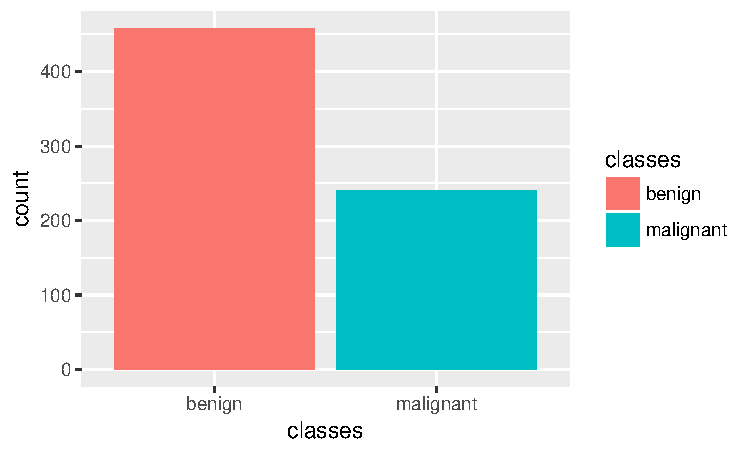
\includegraphics{webinar_code_files/figure-latex/response_classification-1.pdf}

\begin{itemize}
\tightlist
\item
  Response variable for regression
\end{itemize}

\begin{Shaded}
\begin{Highlighting}[]
\KeywordTok{ggplot}\NormalTok{(bc_data, }\KeywordTok{aes}\NormalTok{(}\DataTypeTok{x =} \NormalTok{clump_thickness)) +}
\StringTok{  }\KeywordTok{geom_histogram}\NormalTok{(}\DataTypeTok{bins =} \DecValTok{10}\NormalTok{)}
\end{Highlighting}
\end{Shaded}

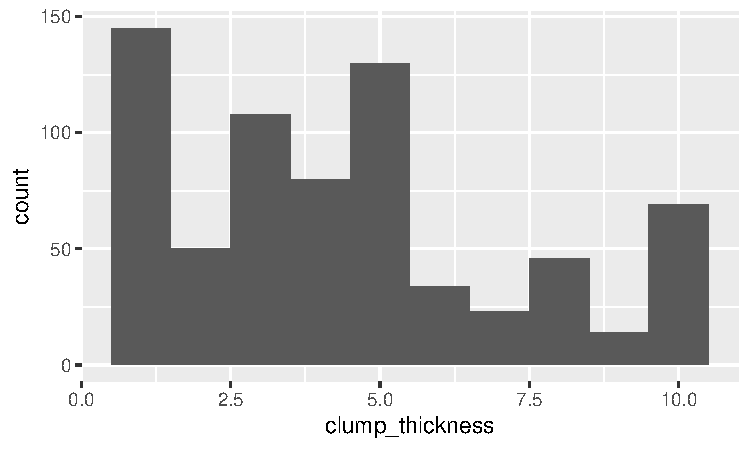
\includegraphics{webinar_code_files/figure-latex/response_regression-1.pdf}

\begin{itemize}
\tightlist
\item
  Principal Component Analysis
\end{itemize}

To get an idea about the dimensionality and variance of the datasets, I
am first looking at PCA plots for samples and features. The first two
principal components (PCs) show the two components that explain the
majority of variation in the data.

\begin{Shaded}
\begin{Highlighting}[]
\KeywordTok{library}\NormalTok{(pcaGoPromoter)}
\KeywordTok{library}\NormalTok{(ellipse)}

\CommentTok{# perform pca and extract scores}
\NormalTok{pcaOutput <-}\StringTok{ }\KeywordTok{pca}\NormalTok{(}\KeywordTok{t}\NormalTok{(bc_data[, -}\DecValTok{1}\NormalTok{]), }\DataTypeTok{printDropped =} \OtherTok{FALSE}\NormalTok{, }\DataTypeTok{scale =} \OtherTok{TRUE}\NormalTok{, }\DataTypeTok{center =} \OtherTok{TRUE}\NormalTok{)}
\NormalTok{pcaOutput2 <-}\StringTok{ }\KeywordTok{as.data.frame}\NormalTok{(pcaOutput$scores)}
  
\CommentTok{# define groups for plotting}
\NormalTok{pcaOutput2$groups <-}\StringTok{ }\NormalTok{bc_data$classes}
  
\NormalTok{centroids <-}\StringTok{ }\KeywordTok{aggregate}\NormalTok{(}\KeywordTok{cbind}\NormalTok{(PC1, PC2) ~}\StringTok{ }\NormalTok{groups, pcaOutput2, mean)}

\NormalTok{conf.rgn  <-}\StringTok{ }\KeywordTok{do.call}\NormalTok{(rbind, }\KeywordTok{lapply}\NormalTok{(}\KeywordTok{unique}\NormalTok{(pcaOutput2$groups), function(t)}
  \KeywordTok{data.frame}\NormalTok{(}\DataTypeTok{groups =} \KeywordTok{as.character}\NormalTok{(t),}
             \KeywordTok{ellipse}\NormalTok{(}\KeywordTok{cov}\NormalTok{(pcaOutput2[pcaOutput2$groups ==}\StringTok{ }\NormalTok{t, }\DecValTok{1}\NormalTok{:}\DecValTok{2}\NormalTok{]),}
                   \DataTypeTok{centre =} \KeywordTok{as.matrix}\NormalTok{(centroids[centroids$groups ==}\StringTok{ }\NormalTok{t, }\DecValTok{2}\NormalTok{:}\DecValTok{3}\NormalTok{]),}
                   \DataTypeTok{level =} \FloatTok{0.95}\NormalTok{),}
             \DataTypeTok{stringsAsFactors =} \OtherTok{FALSE}\NormalTok{)))}
    
\KeywordTok{ggplot}\NormalTok{(}\DataTypeTok{data =} \NormalTok{pcaOutput2, }\KeywordTok{aes}\NormalTok{(}\DataTypeTok{x =} \NormalTok{PC1, }\DataTypeTok{y =} \NormalTok{PC2, }\DataTypeTok{group =} \NormalTok{groups, }\DataTypeTok{color =} \NormalTok{groups)) +}\StringTok{ }
\StringTok{    }\KeywordTok{geom_polygon}\NormalTok{(}\DataTypeTok{data =} \NormalTok{conf.rgn, }\KeywordTok{aes}\NormalTok{(}\DataTypeTok{fill =} \NormalTok{groups), }\DataTypeTok{alpha =} \FloatTok{0.2}\NormalTok{) +}
\StringTok{    }\KeywordTok{geom_point}\NormalTok{(}\DataTypeTok{size =} \DecValTok{2}\NormalTok{, }\DataTypeTok{alpha =} \FloatTok{0.6}\NormalTok{) +}\StringTok{ }
\StringTok{    }\KeywordTok{scale_color_brewer}\NormalTok{(}\DataTypeTok{palette =} \StringTok{"Set1"}\NormalTok{) +}
\StringTok{    }\KeywordTok{labs}\NormalTok{(}\DataTypeTok{color =} \StringTok{""}\NormalTok{,}
         \DataTypeTok{fill =} \StringTok{""}\NormalTok{,}
         \DataTypeTok{x =} \KeywordTok{paste0}\NormalTok{(}\StringTok{"PC1: "}\NormalTok{, }\KeywordTok{round}\NormalTok{(pcaOutput$pov[}\DecValTok{1}\NormalTok{], }\DataTypeTok{digits =} \DecValTok{2}\NormalTok{) *}\StringTok{ }\DecValTok{100}\NormalTok{, }\StringTok{"% variance"}\NormalTok{),}
         \DataTypeTok{y =} \KeywordTok{paste0}\NormalTok{(}\StringTok{"PC2: "}\NormalTok{, }\KeywordTok{round}\NormalTok{(pcaOutput$pov[}\DecValTok{2}\NormalTok{], }\DataTypeTok{digits =} \DecValTok{2}\NormalTok{) *}\StringTok{ }\DecValTok{100}\NormalTok{, }\StringTok{"% variance"}\NormalTok{)) }
\end{Highlighting}
\end{Shaded}

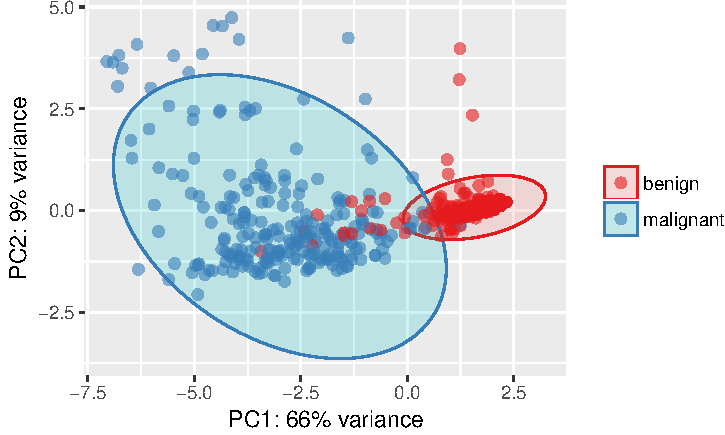
\includegraphics{webinar_code_files/figure-latex/pca-1.pdf}

\begin{itemize}
\tightlist
\item
  Features
\end{itemize}

\begin{Shaded}
\begin{Highlighting}[]
\KeywordTok{library}\NormalTok{(tidyr)}
\end{Highlighting}
\end{Shaded}

\begin{verbatim}
## 
## Attaching package: 'tidyr'
\end{verbatim}

\begin{verbatim}
## The following object is masked from 'package:S4Vectors':
## 
##     expand
\end{verbatim}

\begin{Shaded}
\begin{Highlighting}[]
\KeywordTok{gather}\NormalTok{(bc_data, x, y, clump_thickness:mitosis) %>%}
\StringTok{  }\KeywordTok{ggplot}\NormalTok{(}\KeywordTok{aes}\NormalTok{(}\DataTypeTok{x =} \NormalTok{y, }\DataTypeTok{color =} \NormalTok{classes, }\DataTypeTok{fill =} \NormalTok{classes)) +}
\StringTok{    }\KeywordTok{geom_density}\NormalTok{(}\DataTypeTok{alpha =} \FloatTok{0.3}\NormalTok{) +}
\StringTok{    }\KeywordTok{facet_wrap}\NormalTok{( ~}\StringTok{ }\NormalTok{x, }\DataTypeTok{scales =} \StringTok{"free"}\NormalTok{, }\DataTypeTok{ncol =} \DecValTok{3}\NormalTok{)}
\end{Highlighting}
\end{Shaded}

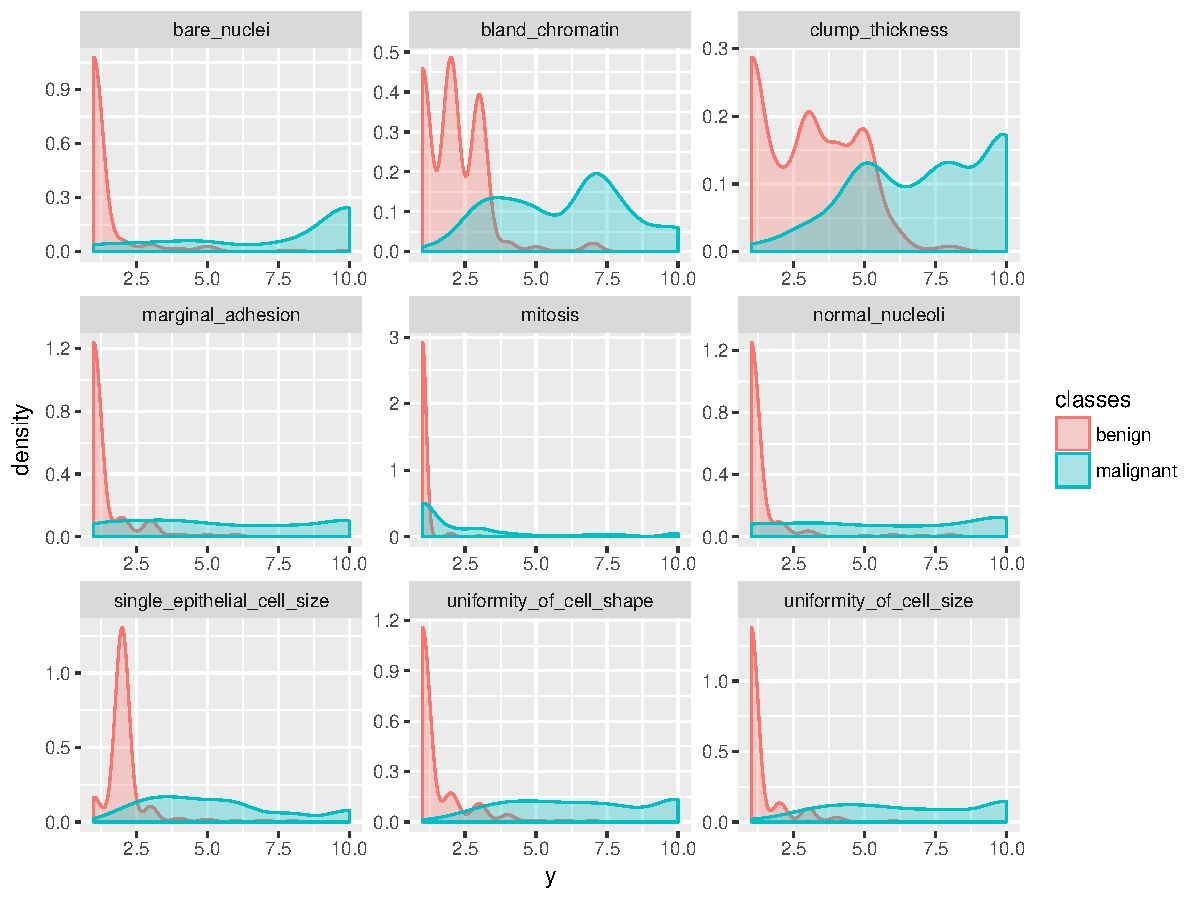
\includegraphics{webinar_code_files/figure-latex/features-1.pdf}

\subsection{Machine Learning packages for
R}\label{machine-learning-packages-for-r}

\subsubsection{\texorpdfstring{\href{http://topepo.github.io/caret/index.html}{caret}}{caret}}\label{caret}

\begin{Shaded}
\begin{Highlighting}[]
\KeywordTok{library}\NormalTok{(caret)}
\end{Highlighting}
\end{Shaded}

\paragraph{Training, validation and test
data}\label{training-validation-and-test-data}

\begin{Shaded}
\begin{Highlighting}[]
\KeywordTok{set.seed}\NormalTok{(}\DecValTok{42}\NormalTok{)}
\NormalTok{index <-}\StringTok{ }\KeywordTok{createDataPartition}\NormalTok{(bc_data$classes, }\DataTypeTok{p =} \FloatTok{0.7}\NormalTok{, }\DataTypeTok{list =} \OtherTok{FALSE}\NormalTok{)}
\NormalTok{train_data <-}\StringTok{ }\NormalTok{bc_data[index, ]}
\NormalTok{test_data  <-}\StringTok{ }\NormalTok{bc_data[-index, ]}
\end{Highlighting}
\end{Shaded}

\begin{Shaded}
\begin{Highlighting}[]
\KeywordTok{library}\NormalTok{(dplyr)}

\KeywordTok{rbind}\NormalTok{(}\KeywordTok{data.frame}\NormalTok{(}\DataTypeTok{group =} \StringTok{"train"}\NormalTok{, train_data),}
      \KeywordTok{data.frame}\NormalTok{(}\DataTypeTok{group =} \StringTok{"test"}\NormalTok{, test_data)) %>%}
\StringTok{  }\KeywordTok{gather}\NormalTok{(x, y, clump_thickness:mitosis) %>%}
\StringTok{  }\KeywordTok{ggplot}\NormalTok{(}\KeywordTok{aes}\NormalTok{(}\DataTypeTok{x =} \NormalTok{y, }\DataTypeTok{color =} \NormalTok{group, }\DataTypeTok{fill =} \NormalTok{group)) +}
\StringTok{    }\KeywordTok{geom_density}\NormalTok{(}\DataTypeTok{alpha =} \FloatTok{0.3}\NormalTok{) +}
\StringTok{    }\KeywordTok{facet_wrap}\NormalTok{( ~}\StringTok{ }\NormalTok{x, }\DataTypeTok{scales =} \StringTok{"free"}\NormalTok{, }\DataTypeTok{ncol =} \DecValTok{3}\NormalTok{)}
\end{Highlighting}
\end{Shaded}

\begin{center}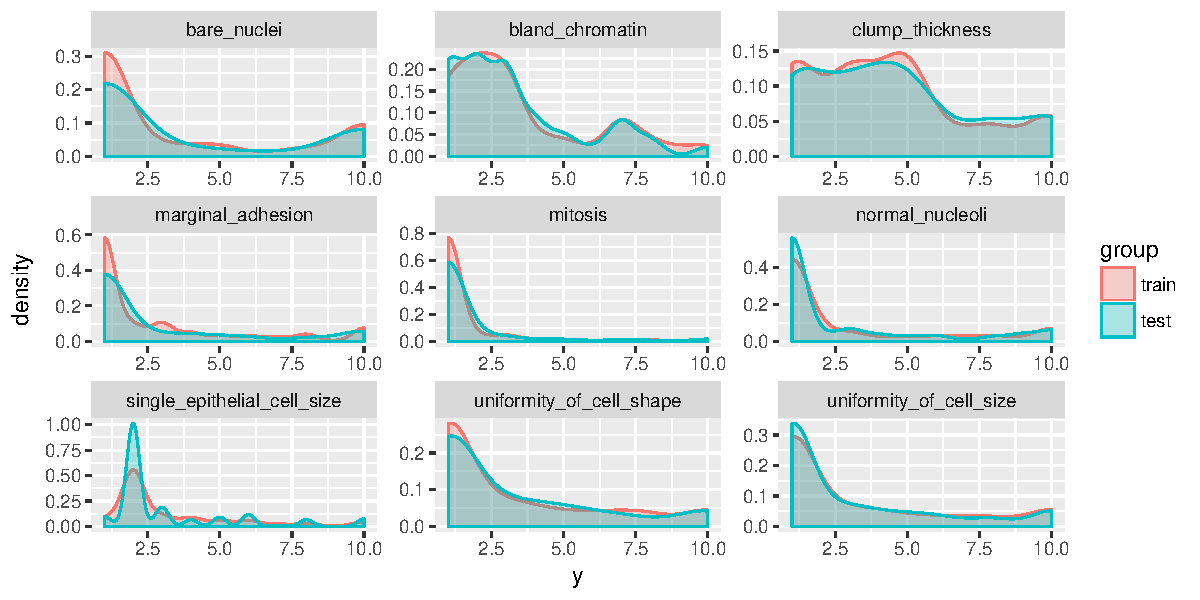
\includegraphics{webinar_code_files/figure-latex/distribution-1} \end{center}

\paragraph{Classification}\label{classification}

\subparagraph{Decision trees}\label{decision-trees}

\href{https://cran.r-project.org/web/packages/rpart/rpart.pdf}{rpart}

\begin{Shaded}
\begin{Highlighting}[]
\KeywordTok{library}\NormalTok{(rpart)}
\KeywordTok{library}\NormalTok{(rpart.plot)}

\KeywordTok{set.seed}\NormalTok{(}\DecValTok{42}\NormalTok{)}
\NormalTok{fit <-}\StringTok{ }\KeywordTok{rpart}\NormalTok{(classes ~}\StringTok{ }\NormalTok{.,}
            \DataTypeTok{data =} \NormalTok{train_data,}
            \DataTypeTok{method =} \StringTok{"class"}\NormalTok{,}
            \DataTypeTok{control =} \KeywordTok{rpart.control}\NormalTok{(}\DataTypeTok{xval =} \DecValTok{10}\NormalTok{, }
                                    \DataTypeTok{minbucket =} \DecValTok{2}\NormalTok{, }
                                    \DataTypeTok{cp =} \DecValTok{0}\NormalTok{), }
             \DataTypeTok{parms =} \KeywordTok{list}\NormalTok{(}\DataTypeTok{split =} \StringTok{"information"}\NormalTok{))}

\KeywordTok{rpart.plot}\NormalTok{(fit, }\DataTypeTok{extra =} \DecValTok{100}\NormalTok{)}
\end{Highlighting}
\end{Shaded}

\begin{center}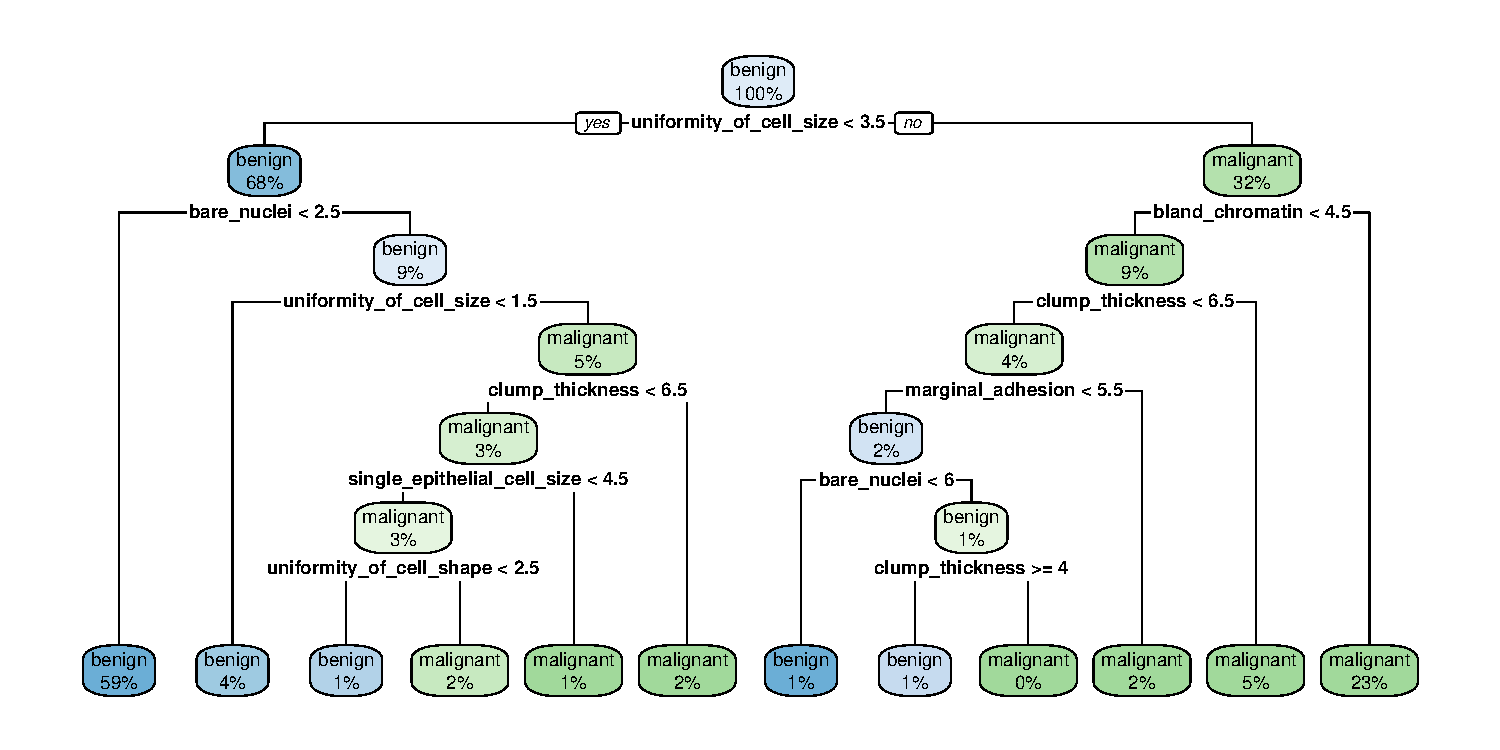
\includegraphics{webinar_code_files/figure-latex/decision_tree-1} \end{center}

\subparagraph{Random Forests}\label{random-forests}

\href{https://www.stat.berkeley.edu/~breiman/RandomForests/cc_home.htm}{Random
Forests} predictions are based on the generation of multiple
classification trees. Can be used for classification and regression
tasks. Here, I show a classification task.

\begin{Shaded}
\begin{Highlighting}[]
\KeywordTok{set.seed}\NormalTok{(}\DecValTok{42}\NormalTok{)}
\NormalTok{model_rf <-}\StringTok{ }\NormalTok{caret::}\KeywordTok{train}\NormalTok{(classes ~}\StringTok{ }\NormalTok{.,}
                         \DataTypeTok{data =} \NormalTok{train_data,}
                         \DataTypeTok{method =} \StringTok{"rf"}\NormalTok{,}
                         \DataTypeTok{preProcess =} \KeywordTok{c}\NormalTok{(}\StringTok{"scale"}\NormalTok{, }\StringTok{"center"}\NormalTok{),}
                         \DataTypeTok{trControl =} \KeywordTok{trainControl}\NormalTok{(}\DataTypeTok{method =} \StringTok{"repeatedcv"}\NormalTok{, }
                                                  \DataTypeTok{number =} \DecValTok{10}\NormalTok{, }
                                                  \DataTypeTok{repeats =} \DecValTok{10}\NormalTok{, }
                                                  \DataTypeTok{savePredictions =} \OtherTok{TRUE}\NormalTok{, }
                                                  \DataTypeTok{verboseIter =} \OtherTok{FALSE}\NormalTok{))}
\end{Highlighting}
\end{Shaded}

When you specify \texttt{savePredictions\ =\ TRUE}, you can access the
cross-validation resuls with \texttt{model\_rf\$pred}.

\begin{Shaded}
\begin{Highlighting}[]
\NormalTok{model_rf}
\end{Highlighting}
\end{Shaded}

\begin{verbatim}
## Random Forest 
## 
## 490 samples
##   9 predictor
##   2 classes: 'benign', 'malignant' 
## 
## Pre-processing: scaled (9), centered (9) 
## Resampling: Cross-Validated (10 fold, repeated 10 times) 
## Summary of sample sizes: 442, 441, 441, 441, 441, 441, ... 
## Resampling results across tuning parameters:
## 
##   mtry  Accuracy   Kappa    
##   2     0.9706276  0.9354524
##   5     0.9665454  0.9261717
##   9     0.9630759  0.9180675
## 
## Accuracy was used to select the optimal model using  the largest value.
## The final value used for the model was mtry = 2.
\end{verbatim}

\begin{Shaded}
\begin{Highlighting}[]
\NormalTok{model_rf$finalModel$confusion}
\end{Highlighting}
\end{Shaded}

\begin{verbatim}
##           benign malignant class.error
## benign       313         8  0.02492212
## malignant      4       165  0.02366864
\end{verbatim}

\begin{itemize}
\tightlist
\item
  Feature Importance
\end{itemize}

\begin{Shaded}
\begin{Highlighting}[]
\NormalTok{imp <-}\StringTok{ }\NormalTok{model_rf$finalModel$importance}
\NormalTok{imp[}\KeywordTok{order}\NormalTok{(imp, }\DataTypeTok{decreasing =} \OtherTok{TRUE}\NormalTok{), ]}
\end{Highlighting}
\end{Shaded}

\begin{verbatim}
##     uniformity_of_cell_size    uniformity_of_cell_shape 
##                   54.416003                   41.553022 
##             bland_chromatin                 bare_nuclei 
##                   29.343027                   28.483842 
##             normal_nucleoli single_epithelial_cell_size 
##                   19.239635                   18.480155 
##             clump_thickness           marginal_adhesion 
##                   13.276702                   12.143355 
##                     mitosis 
##                    3.081635
\end{verbatim}

\begin{Shaded}
\begin{Highlighting}[]
\CommentTok{# estimate variable importance}
\NormalTok{importance <-}\StringTok{ }\KeywordTok{varImp}\NormalTok{(model_rf, }\DataTypeTok{scale =} \OtherTok{TRUE}\NormalTok{)}
\KeywordTok{plot}\NormalTok{(importance)}
\end{Highlighting}
\end{Shaded}

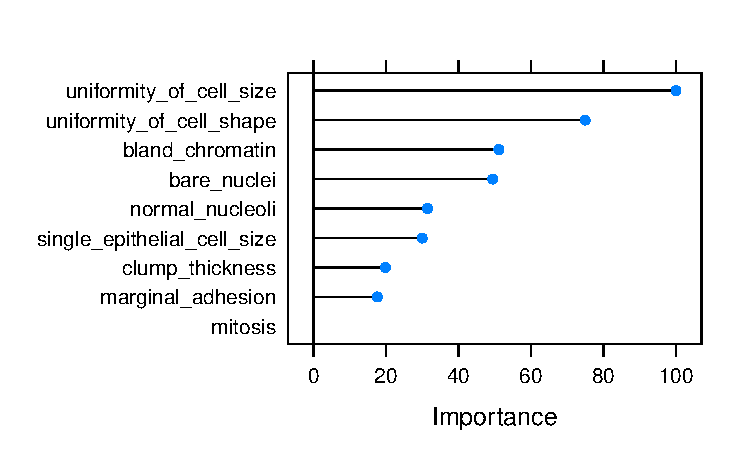
\includegraphics{webinar_code_files/figure-latex/importance_rf-1.pdf}

\begin{itemize}
\tightlist
\item
  predicting test data
\end{itemize}

\begin{Shaded}
\begin{Highlighting}[]
\KeywordTok{confusionMatrix}\NormalTok{(}\KeywordTok{predict}\NormalTok{(model_rf, test_data), test_data$classes)}
\end{Highlighting}
\end{Shaded}

\begin{verbatim}
## Confusion Matrix and Statistics
## 
##            Reference
## Prediction  benign malignant
##   benign       133         2
##   malignant      4        70
##                                           
##                Accuracy : 0.9713          
##                  95% CI : (0.9386, 0.9894)
##     No Information Rate : 0.6555          
##     P-Value [Acc > NIR] : <2e-16          
##                                           
##                   Kappa : 0.9369          
##  Mcnemar's Test P-Value : 0.6831          
##                                           
##             Sensitivity : 0.9708          
##             Specificity : 0.9722          
##          Pos Pred Value : 0.9852          
##          Neg Pred Value : 0.9459          
##              Prevalence : 0.6555          
##          Detection Rate : 0.6364          
##    Detection Prevalence : 0.6459          
##       Balanced Accuracy : 0.9715          
##                                           
##        'Positive' Class : benign          
## 
\end{verbatim}

\begin{Shaded}
\begin{Highlighting}[]
\NormalTok{results <-}\StringTok{ }\KeywordTok{data.frame}\NormalTok{(}\DataTypeTok{actual =} \NormalTok{test_data$classes,}
                      \KeywordTok{predict}\NormalTok{(model_rf, test_data, }\DataTypeTok{type =} \StringTok{"prob"}\NormalTok{))}

\NormalTok{results$prediction <-}\StringTok{ }\KeywordTok{ifelse}\NormalTok{(results$benign >}\StringTok{ }\FloatTok{0.5}\NormalTok{, }\StringTok{"benign"}\NormalTok{,}
                             \KeywordTok{ifelse}\NormalTok{(results$malignant >}\StringTok{ }\FloatTok{0.5}\NormalTok{, }\StringTok{"malignant"}\NormalTok{, }\OtherTok{NA}\NormalTok{))}

\NormalTok{results$correct <-}\StringTok{ }\KeywordTok{ifelse}\NormalTok{(results$actual ==}\StringTok{ }\NormalTok{results$prediction, }\OtherTok{TRUE}\NormalTok{, }\OtherTok{FALSE}\NormalTok{)}

\KeywordTok{ggplot}\NormalTok{(results, }\KeywordTok{aes}\NormalTok{(}\DataTypeTok{x =} \NormalTok{prediction, }\DataTypeTok{fill =} \NormalTok{correct)) +}
\StringTok{  }\KeywordTok{geom_bar}\NormalTok{(}\DataTypeTok{position =} \StringTok{"dodge"}\NormalTok{)}
\end{Highlighting}
\end{Shaded}

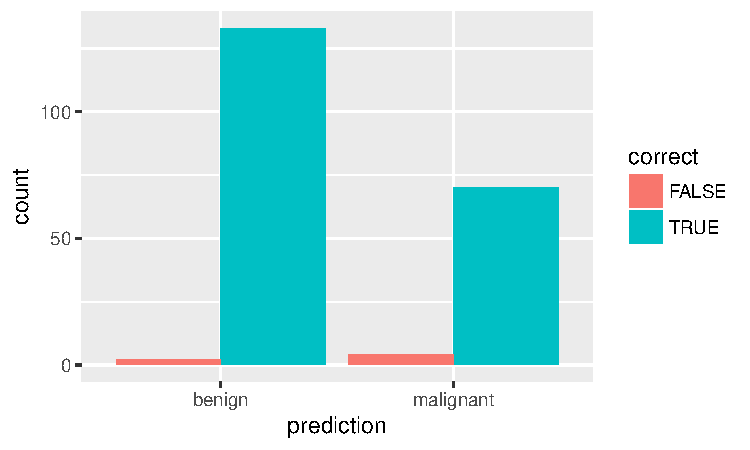
\includegraphics{webinar_code_files/figure-latex/results_bar_rf-1.pdf}

\begin{Shaded}
\begin{Highlighting}[]
\KeywordTok{ggplot}\NormalTok{(results, }\KeywordTok{aes}\NormalTok{(}\DataTypeTok{x =} \NormalTok{prediction, }\DataTypeTok{y =} \NormalTok{benign, }\DataTypeTok{color =} \NormalTok{correct, }\DataTypeTok{shape =} \NormalTok{correct)) +}
\StringTok{  }\KeywordTok{geom_jitter}\NormalTok{(}\DataTypeTok{size =} \DecValTok{3}\NormalTok{, }\DataTypeTok{alpha =} \FloatTok{0.6}\NormalTok{)}
\end{Highlighting}
\end{Shaded}

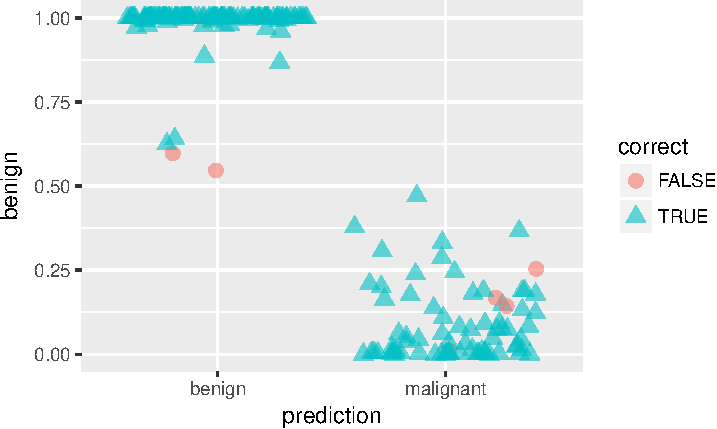
\includegraphics{webinar_code_files/figure-latex/results_jitter_rf-1.pdf}

\subparagraph{Extreme gradient boosting
trees}\label{extreme-gradient-boosting-trees}

\href{http://xgboost.readthedocs.io/en/latest/model.html}{Extreme
gradient boosting (XGBoost)} is a faster and improved implementation of
\href{https://en.wikipedia.org/wiki/Gradient_boosting}{gradient
boosting} for supervised learning.

\begin{quote}
``XGBoost uses a more regularized model formalization to control
over-fitting, which gives it better performance.'' Tianqi Chen,
developer of xgboost
\end{quote}

XGBoost is a tree ensemble model, which means the sum of predictions
from a set of classification and regression trees (CART). In that,
XGBoost is similar to Random Forests but it uses a different approach to
model training. Can be used for classification and regression tasks.
Here, I show a classification task.

\begin{Shaded}
\begin{Highlighting}[]
\KeywordTok{set.seed}\NormalTok{(}\DecValTok{42}\NormalTok{)}
\NormalTok{model_xgb <-}\StringTok{ }\NormalTok{caret::}\KeywordTok{train}\NormalTok{(classes ~}\StringTok{ }\NormalTok{.,}
                          \DataTypeTok{data =} \NormalTok{train_data,}
                          \DataTypeTok{method =} \StringTok{"xgbTree"}\NormalTok{,}
                          \DataTypeTok{preProcess =} \KeywordTok{c}\NormalTok{(}\StringTok{"scale"}\NormalTok{, }\StringTok{"center"}\NormalTok{),}
                          \DataTypeTok{trControl =} \KeywordTok{trainControl}\NormalTok{(}\DataTypeTok{method =} \StringTok{"repeatedcv"}\NormalTok{, }
                                                  \DataTypeTok{number =} \DecValTok{10}\NormalTok{, }
                                                  \DataTypeTok{repeats =} \DecValTok{10}\NormalTok{, }
                                                  \DataTypeTok{savePredictions =} \OtherTok{TRUE}\NormalTok{, }
                                                  \DataTypeTok{verboseIter =} \OtherTok{FALSE}\NormalTok{))}
\end{Highlighting}
\end{Shaded}

\begin{itemize}
\tightlist
\item
  Feature Importance
\end{itemize}

\begin{Shaded}
\begin{Highlighting}[]
\NormalTok{importance <-}\StringTok{ }\KeywordTok{varImp}\NormalTok{(model_xgb, }\DataTypeTok{scale =} \OtherTok{TRUE}\NormalTok{)}
\KeywordTok{plot}\NormalTok{(importance)}
\end{Highlighting}
\end{Shaded}

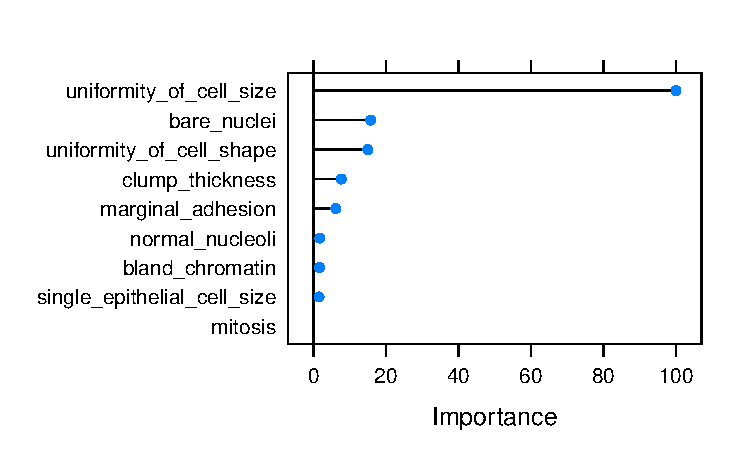
\includegraphics{webinar_code_files/figure-latex/importance_xgb-1.pdf}

\begin{itemize}
\tightlist
\item
  predicting test data
\end{itemize}

\begin{Shaded}
\begin{Highlighting}[]
\KeywordTok{confusionMatrix}\NormalTok{(}\KeywordTok{predict}\NormalTok{(model_xgb, test_data), test_data$classes)}
\end{Highlighting}
\end{Shaded}

\begin{verbatim}
## Confusion Matrix and Statistics
## 
##            Reference
## Prediction  benign malignant
##   benign       132         2
##   malignant      5        70
##                                           
##                Accuracy : 0.9665          
##                  95% CI : (0.9322, 0.9864)
##     No Information Rate : 0.6555          
##     P-Value [Acc > NIR] : <2e-16          
##                                           
##                   Kappa : 0.9266          
##  Mcnemar's Test P-Value : 0.4497          
##                                           
##             Sensitivity : 0.9635          
##             Specificity : 0.9722          
##          Pos Pred Value : 0.9851          
##          Neg Pred Value : 0.9333          
##              Prevalence : 0.6555          
##          Detection Rate : 0.6316          
##    Detection Prevalence : 0.6411          
##       Balanced Accuracy : 0.9679          
##                                           
##        'Positive' Class : benign          
## 
\end{verbatim}

\begin{Shaded}
\begin{Highlighting}[]
\NormalTok{results <-}\StringTok{ }\KeywordTok{data.frame}\NormalTok{(}\DataTypeTok{actual =} \NormalTok{test_data$classes,}
                      \KeywordTok{predict}\NormalTok{(model_xgb, test_data, }\DataTypeTok{type =} \StringTok{"prob"}\NormalTok{))}

\NormalTok{results$prediction <-}\StringTok{ }\KeywordTok{ifelse}\NormalTok{(results$benign >}\StringTok{ }\FloatTok{0.5}\NormalTok{, }\StringTok{"benign"}\NormalTok{,}
                             \KeywordTok{ifelse}\NormalTok{(results$malignant >}\StringTok{ }\FloatTok{0.5}\NormalTok{, }\StringTok{"malignant"}\NormalTok{, }\OtherTok{NA}\NormalTok{))}

\NormalTok{results$correct <-}\StringTok{ }\KeywordTok{ifelse}\NormalTok{(results$actual ==}\StringTok{ }\NormalTok{results$prediction, }\OtherTok{TRUE}\NormalTok{, }\OtherTok{FALSE}\NormalTok{)}

\KeywordTok{ggplot}\NormalTok{(results, }\KeywordTok{aes}\NormalTok{(}\DataTypeTok{x =} \NormalTok{prediction, }\DataTypeTok{fill =} \NormalTok{correct)) +}
\StringTok{  }\KeywordTok{geom_bar}\NormalTok{(}\DataTypeTok{position =} \StringTok{"dodge"}\NormalTok{)}
\end{Highlighting}
\end{Shaded}

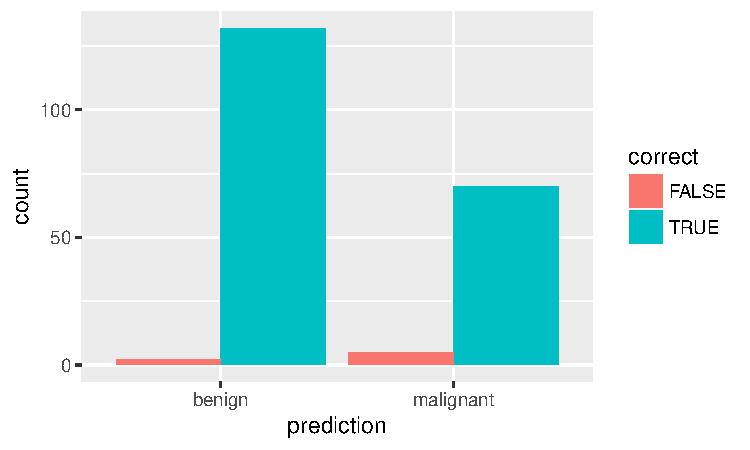
\includegraphics{webinar_code_files/figure-latex/results_bar_xgb-1.pdf}

\begin{Shaded}
\begin{Highlighting}[]
\KeywordTok{ggplot}\NormalTok{(results, }\KeywordTok{aes}\NormalTok{(}\DataTypeTok{x =} \NormalTok{prediction, }\DataTypeTok{y =} \NormalTok{benign, }\DataTypeTok{color =} \NormalTok{correct, }\DataTypeTok{shape =} \NormalTok{correct)) +}
\StringTok{  }\KeywordTok{geom_jitter}\NormalTok{(}\DataTypeTok{size =} \DecValTok{3}\NormalTok{, }\DataTypeTok{alpha =} \FloatTok{0.6}\NormalTok{)}
\end{Highlighting}
\end{Shaded}

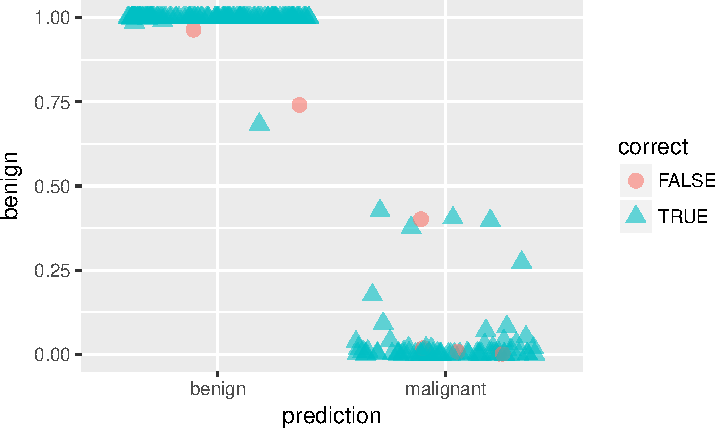
\includegraphics{webinar_code_files/figure-latex/results_jitter_xgb-1.pdf}

\paragraph{Regression}\label{regression}

\begin{Shaded}
\begin{Highlighting}[]
\KeywordTok{set.seed}\NormalTok{(}\DecValTok{42}\NormalTok{)}
\NormalTok{model_glm <-}\StringTok{ }\NormalTok{caret::}\KeywordTok{train}\NormalTok{(clump_thickness ~}\StringTok{ }\NormalTok{.,}
                          \DataTypeTok{data =} \NormalTok{train_data,}
                          \DataTypeTok{method =} \StringTok{"glm"}\NormalTok{,}
                          \DataTypeTok{preProcess =} \KeywordTok{c}\NormalTok{(}\StringTok{"scale"}\NormalTok{, }\StringTok{"center"}\NormalTok{),}
                          \DataTypeTok{trControl =} \KeywordTok{trainControl}\NormalTok{(}\DataTypeTok{method =} \StringTok{"repeatedcv"}\NormalTok{, }
                                                  \DataTypeTok{number =} \DecValTok{10}\NormalTok{, }
                                                  \DataTypeTok{repeats =} \DecValTok{10}\NormalTok{, }
                                                  \DataTypeTok{savePredictions =} \OtherTok{TRUE}\NormalTok{, }
                                                  \DataTypeTok{verboseIter =} \OtherTok{FALSE}\NormalTok{))}
\end{Highlighting}
\end{Shaded}

\begin{Shaded}
\begin{Highlighting}[]
\NormalTok{model_glm}
\end{Highlighting}
\end{Shaded}

\begin{verbatim}
## Generalized Linear Model 
## 
## 490 samples
##   9 predictor
## 
## Pre-processing: scaled (9), centered (9) 
## Resampling: Cross-Validated (10 fold, repeated 10 times) 
## Summary of sample sizes: 441, 441, 440, 442, 441, 440, ... 
## Resampling results:
## 
##   RMSE      Rsquared 
##   1.974296  0.5016141
## 
## 
\end{verbatim}

\begin{Shaded}
\begin{Highlighting}[]
\KeywordTok{data.frame}\NormalTok{(}\DataTypeTok{actual =} \NormalTok{test_data$clump_thickness,}
           \DataTypeTok{predicted =} \KeywordTok{predict}\NormalTok{(model_glm, test_data)) %>%}
\StringTok{  }\KeywordTok{ggplot}\NormalTok{(}\KeywordTok{aes}\NormalTok{(}\DataTypeTok{x =} \NormalTok{actual, }\DataTypeTok{y =} \NormalTok{predicted)) +}
\StringTok{    }\KeywordTok{geom_jitter}\NormalTok{() +}
\StringTok{    }\KeywordTok{geom_smooth}\NormalTok{(}\DataTypeTok{method =} \StringTok{"lm"}\NormalTok{)}
\end{Highlighting}
\end{Shaded}

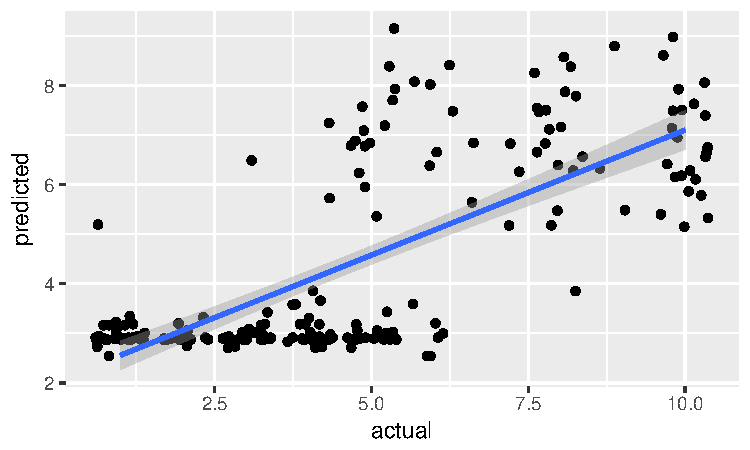
\includegraphics{webinar_code_files/figure-latex/regression_result-1.pdf}

\subsubsection{Feature Selection}\label{feature-selection}

Machine learning uses so called features (i.e.~variables or attributes)
to generate predictive models. Using a suitable combination of features
is essential for obtaining high precision and accuracy. Because too many
(unspecific) features pose the problem of overfitting the model, we
generally want to restrict the features in our models to those, that are
most relevant for the response variable we want to predict. Using as few
features as possible will also reduce the complexity of our models,
which means it needs less time and computer power to run and is easier
to understand.

Performing feature selection on the whole dataset would lead to
prediction bias, we therefore need to run the whole modeling process on
the training data alone!

\begin{itemize}
\tightlist
\item
  Correlation
\end{itemize}

Often we have features that are highly correlated and thus provide
redundant information. By eliminating highly correlated features we can
avoid a predictive bias for the information contained in these features.
This also shows us, that when we want to make statements about the
biological/ medical importance of specific features, we need to keep in
mind that just because they are suitable to predicting an outcome they
are not necessarily causal - they could simply be correlated with causal
factors.

Correlations between all features are calculated and visualised with the
\emph{corrplot} package. I am then removing all features with a
correlation higher than 0.7, keeping the feature with the lower mean.

\begin{Shaded}
\begin{Highlighting}[]
\KeywordTok{library}\NormalTok{(corrplot)}

\CommentTok{# calculate correlation matrix}
\NormalTok{corMatMy <-}\StringTok{ }\KeywordTok{cor}\NormalTok{(train_data[, -}\DecValTok{1}\NormalTok{])}
\KeywordTok{corrplot}\NormalTok{(corMatMy, }\DataTypeTok{order =} \StringTok{"hclust"}\NormalTok{)}
\end{Highlighting}
\end{Shaded}

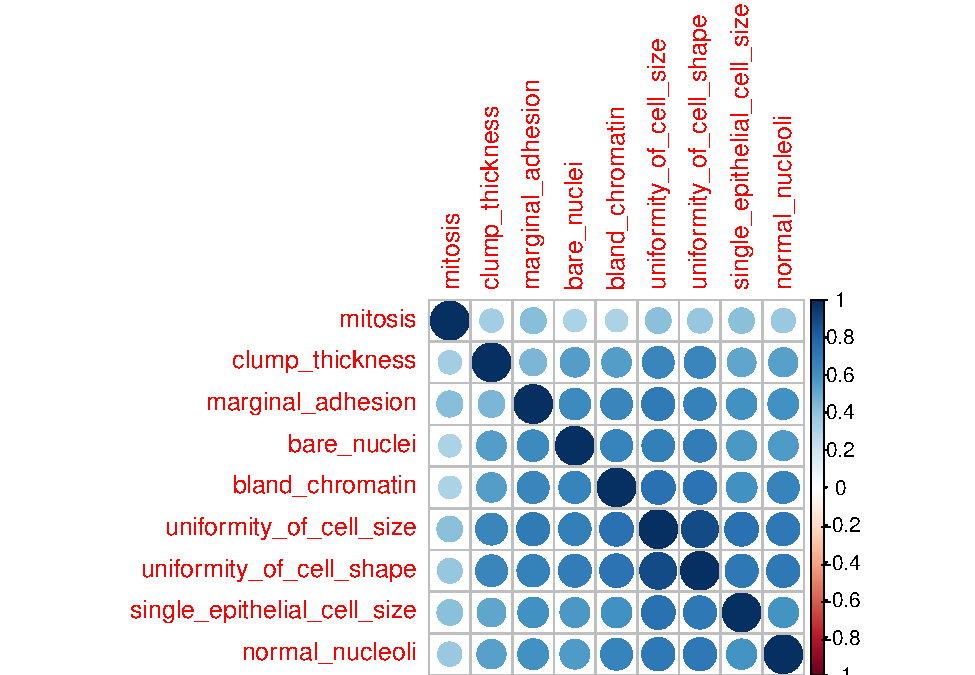
\includegraphics{webinar_code_files/figure-latex/unnamed-chunk-24-1.pdf}

\begin{Shaded}
\begin{Highlighting}[]
\CommentTok{#Apply correlation filter at 0.70,}
\NormalTok{highlyCor <-}\StringTok{ }\KeywordTok{colnames}\NormalTok{(train_data[, -}\DecValTok{1}\NormalTok{])[}\KeywordTok{findCorrelation}\NormalTok{(corMatMy, }\DataTypeTok{cutoff =} \FloatTok{0.7}\NormalTok{, }\DataTypeTok{verbose =} \OtherTok{TRUE}\NormalTok{)]}
\end{Highlighting}
\end{Shaded}

\begin{verbatim}
## Compare row 2  and column  3 with corr  0.899 
##   Means:  0.696 vs 0.575 so flagging column 2 
## Compare row 3  and column  7 with corr  0.736 
##   Means:  0.654 vs 0.55 so flagging column 3 
## All correlations <= 0.7
\end{verbatim}

\begin{Shaded}
\begin{Highlighting}[]
\CommentTok{# which variables are flagged for removal?}
\NormalTok{highlyCor}
\end{Highlighting}
\end{Shaded}

\begin{verbatim}
## [1] "uniformity_of_cell_size"  "uniformity_of_cell_shape"
\end{verbatim}

\begin{Shaded}
\begin{Highlighting}[]
\CommentTok{#then we remove these variables}
\NormalTok{train_data_cor <-}\StringTok{ }\NormalTok{train_data[, }\KeywordTok{which}\NormalTok{(!}\KeywordTok{colnames}\NormalTok{(train_data) %in%}\StringTok{ }\NormalTok{highlyCor)]}
\end{Highlighting}
\end{Shaded}

\begin{itemize}
\tightlist
\item
  Recursive Feature Elimination (RFE)
\end{itemize}

Another way to choose features is with Recursive Feature Elimination.
RFE uses a Random Forest algorithm to test combinations of features and
rate each with an accuracy score. The combination with the highest score
is usually preferential.

\begin{Shaded}
\begin{Highlighting}[]
\CommentTok{# chosen features}
\KeywordTok{predictors}\NormalTok{(results_rfe)}
\end{Highlighting}
\end{Shaded}

\begin{verbatim}
## [1] "bare_nuclei"                 "uniformity_of_cell_size"    
## [3] "clump_thickness"             "uniformity_of_cell_shape"   
## [5] "bland_chromatin"             "marginal_adhesion"          
## [7] "normal_nucleoli"             "single_epithelial_cell_size"
## [9] "mitosis"
\end{verbatim}

\begin{Shaded}
\begin{Highlighting}[]
\NormalTok{train_data_rfe <-}\StringTok{ }\NormalTok{train_data[, }\KeywordTok{c}\NormalTok{(}\DecValTok{1}\NormalTok{, }\KeywordTok{which}\NormalTok{(}\KeywordTok{colnames}\NormalTok{(train_data) %in%}\StringTok{ }\KeywordTok{predictors}\NormalTok{(results_rfe)))]}
\end{Highlighting}
\end{Shaded}

\begin{itemize}
\tightlist
\item
  Genetic Algorithm (GA)
\end{itemize}

The Genetic Algorithm (GA) has been developed based on evolutionary
principles of natural selection: It aims to optimize a population of
individuals with a given set of genotypes by modeling selection over
time. In each generation (i.e.~iteration), each individual's fitness is
calculated based on their genotypes. Then, the fittest individuals are
chosen to produce the next generation. This subsequent generation of
individuals will have genotypes resulting from (re-) combinations of the
parental alleles. These new genotypes will again determine each
individual's fitness. This selection process is iterated for a specified
number of generations and (ideally) leads to fixation of the fittest
alleles in the gene pool.

This concept of optimization can be applied to non-evolutionary models
as well, like feature selection processes in machine learning.

\begin{Shaded}
\begin{Highlighting}[]
\KeywordTok{plot}\NormalTok{(model_ga) }\CommentTok{# Plot mean fitness (AUC) by generation}
\end{Highlighting}
\end{Shaded}

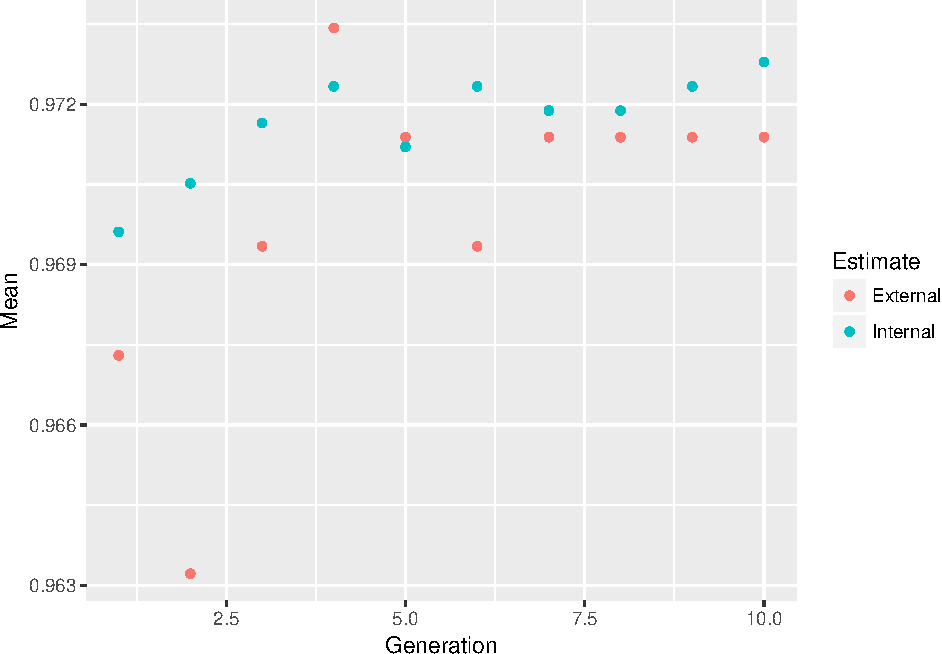
\includegraphics{webinar_code_files/figure-latex/unnamed-chunk-32-1.pdf}

\begin{Shaded}
\begin{Highlighting}[]
\NormalTok{train_data_ga <-}\StringTok{ }\NormalTok{train_data[, }\KeywordTok{c}\NormalTok{(}\DecValTok{1}\NormalTok{, }\KeywordTok{which}\NormalTok{(}\KeywordTok{colnames}\NormalTok{(train_data) %in%}\StringTok{ }\NormalTok{model_ga$ga$final))]}
\end{Highlighting}
\end{Shaded}

\subsubsection{Grid search with h2o}\label{grid-search-with-h2o}

The R package h2o provides a convenient interface to
\href{http://www.h2o.ai/h2o/}{H2O}, which is an open-source machine
learning and deep learning platform. H2O distributes a wide range of
common machine learning algorithms for classification, regression and
deep learning.

\begin{Shaded}
\begin{Highlighting}[]
\KeywordTok{library}\NormalTok{(h2o)}
\KeywordTok{h2o.init}\NormalTok{(}\DataTypeTok{nthreads =} \NormalTok{-}\DecValTok{1}\NormalTok{)}
\end{Highlighting}
\end{Shaded}

\begin{verbatim}
##  Connection successful!
## 
## R is connected to the H2O cluster: 
##     H2O cluster uptime:         1 hours 2 minutes 
##     H2O cluster version:        3.10.3.6 
##     H2O cluster version age:    18 days  
##     H2O cluster name:           H2O_started_from_R_Shirin_gkt508 
##     H2O cluster total nodes:    1 
##     H2O cluster total memory:   1.76 GB 
##     H2O cluster total cores:    2 
##     H2O cluster allowed cores:  2 
##     H2O cluster healthy:        TRUE 
##     H2O Connection ip:          localhost 
##     H2O Connection port:        54321 
##     H2O Connection proxy:       NA 
##     R Version:                  R version 3.3.2 (2016-10-31)
\end{verbatim}

\begin{Shaded}
\begin{Highlighting}[]
\NormalTok{bc_data_hf <-}\StringTok{ }\KeywordTok{as.h2o}\NormalTok{(bc_data)}
\end{Highlighting}
\end{Shaded}

\begin{verbatim}
## 
  |                                                                       
  |                                                                 |   0%
  |                                                                       
  |=================================================================| 100%
\end{verbatim}

We can now access all functions from the \textbf{h2o} package that are
built to work on H2O Frames. A useful such function is
\emph{h2o.describe()}. It is similar to base R's \emph{summary()}
function but outputs many more descriptive measures for our data. To get
a good overview about these measures, I am going to plot them.

\begin{Shaded}
\begin{Highlighting}[]
\KeywordTok{h2o.describe}\NormalTok{(bc_data_hf) %>%}
\StringTok{  }\KeywordTok{gather}\NormalTok{(x, y, Zeros:Sigma) %>%}
\StringTok{  }\KeywordTok{mutate}\NormalTok{(}\DataTypeTok{group =} \KeywordTok{ifelse}\NormalTok{(x %in%}\StringTok{ }\KeywordTok{c}\NormalTok{(}\StringTok{"Min"}\NormalTok{, }\StringTok{"Max"}\NormalTok{, }\StringTok{"Mean"}\NormalTok{), }\StringTok{"min, mean, max"}\NormalTok{, }
                        \KeywordTok{ifelse}\NormalTok{(x %in%}\StringTok{ }\KeywordTok{c}\NormalTok{(}\StringTok{"NegInf"}\NormalTok{, }\StringTok{"PosInf"}\NormalTok{), }\StringTok{"Inf"}\NormalTok{, }\StringTok{"sigma, zeros"}\NormalTok{))) %>%}\StringTok{ }
\StringTok{  }\KeywordTok{ggplot}\NormalTok{(}\KeywordTok{aes}\NormalTok{(}\DataTypeTok{x =} \NormalTok{Label, }\DataTypeTok{y =} \KeywordTok{as.numeric}\NormalTok{(y), }\DataTypeTok{color =} \NormalTok{x)) +}
\StringTok{    }\KeywordTok{geom_point}\NormalTok{(}\DataTypeTok{size =} \DecValTok{4}\NormalTok{, }\DataTypeTok{alpha =} \FloatTok{0.6}\NormalTok{) +}
\StringTok{    }\KeywordTok{scale_color_brewer}\NormalTok{(}\DataTypeTok{palette =} \StringTok{"Set1"}\NormalTok{) +}
\StringTok{    }\KeywordTok{theme}\NormalTok{(}\DataTypeTok{axis.text.x =} \KeywordTok{element_text}\NormalTok{(}\DataTypeTok{angle =} \DecValTok{45}\NormalTok{, }\DataTypeTok{vjust =} \DecValTok{1}\NormalTok{, }\DataTypeTok{hjust =} \DecValTok{1}\NormalTok{)) +}
\StringTok{    }\KeywordTok{facet_grid}\NormalTok{(group ~}\StringTok{ }\NormalTok{., }\DataTypeTok{scales =} \StringTok{"free"}\NormalTok{) +}
\StringTok{    }\KeywordTok{labs}\NormalTok{(}\DataTypeTok{x =} \StringTok{"Feature"}\NormalTok{,}
         \DataTypeTok{y =} \StringTok{"Value"}\NormalTok{,}
         \DataTypeTok{color =} \StringTok{""}\NormalTok{)}
\end{Highlighting}
\end{Shaded}

\begin{center}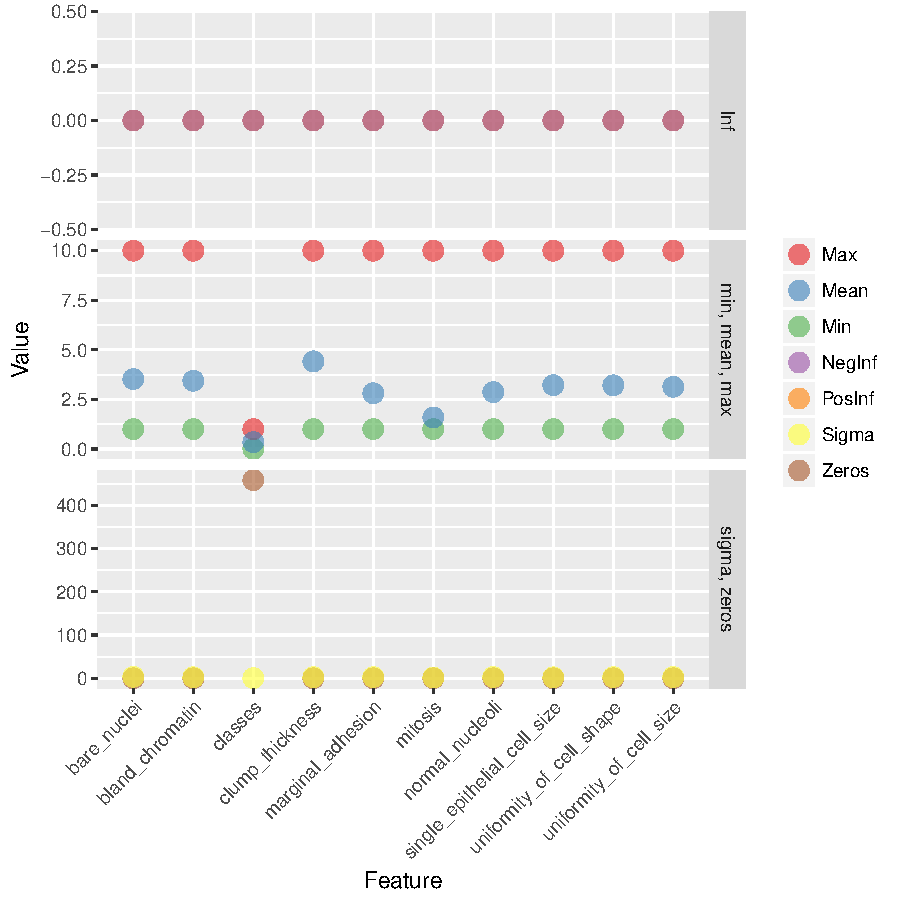
\includegraphics{webinar_code_files/figure-latex/h2o_describe-1} \end{center}

I am also interested in the correlation between features and the output.
We can use the \emph{h2o.cor()} function to calculate the correlation
matrix. It is again much easier to understand the data when we visualize
it, so I am going to create another plot.

\begin{Shaded}
\begin{Highlighting}[]
\KeywordTok{library}\NormalTok{(reshape2) }\CommentTok{# for melting}
\end{Highlighting}
\end{Shaded}

\begin{verbatim}
## 
## Attaching package: 'reshape2'
\end{verbatim}

\begin{verbatim}
## The following object is masked from 'package:tidyr':
## 
##     smiths
\end{verbatim}

\begin{Shaded}
\begin{Highlighting}[]
\NormalTok{bc_data_hf[, }\DecValTok{1}\NormalTok{] <-}\StringTok{ }\KeywordTok{h2o.asfactor}\NormalTok{(bc_data_hf[, }\DecValTok{1}\NormalTok{])}

\NormalTok{cor <-}\StringTok{ }\KeywordTok{h2o.cor}\NormalTok{(bc_data_hf)}
\KeywordTok{rownames}\NormalTok{(cor) <-}\StringTok{ }\KeywordTok{colnames}\NormalTok{(cor)}

\KeywordTok{melt}\NormalTok{(cor) %>%}
\StringTok{  }\KeywordTok{mutate}\NormalTok{(}\DataTypeTok{Var2 =} \KeywordTok{rep}\NormalTok{(}\KeywordTok{rownames}\NormalTok{(cor), }\KeywordTok{nrow}\NormalTok{(cor))) %>%}
\StringTok{  }\KeywordTok{mutate}\NormalTok{(}\DataTypeTok{Var2 =} \KeywordTok{factor}\NormalTok{(Var2, }\DataTypeTok{levels =} \KeywordTok{colnames}\NormalTok{(cor))) %>%}
\StringTok{  }\KeywordTok{mutate}\NormalTok{(}\DataTypeTok{variable =} \KeywordTok{factor}\NormalTok{(variable, }\DataTypeTok{levels =} \KeywordTok{colnames}\NormalTok{(cor))) %>%}
\StringTok{  }\KeywordTok{ggplot}\NormalTok{(}\KeywordTok{aes}\NormalTok{(}\DataTypeTok{x =} \NormalTok{variable, }\DataTypeTok{y =} \NormalTok{Var2, }\DataTypeTok{fill =} \NormalTok{value)) +}\StringTok{ }
\StringTok{    }\KeywordTok{geom_tile}\NormalTok{(}\DataTypeTok{width =} \FloatTok{0.9}\NormalTok{, }\DataTypeTok{height =} \FloatTok{0.9}\NormalTok{) +}
\StringTok{    }\KeywordTok{scale_fill_gradient2}\NormalTok{(}\DataTypeTok{low =} \StringTok{"white"}\NormalTok{, }\DataTypeTok{high =} \StringTok{"red"}\NormalTok{, }\DataTypeTok{name =} \StringTok{"Cor."}\NormalTok{) +}
\StringTok{    }\KeywordTok{theme}\NormalTok{(}\DataTypeTok{axis.text.x =} \KeywordTok{element_text}\NormalTok{(}\DataTypeTok{angle =} \DecValTok{90}\NormalTok{, }\DataTypeTok{vjust =} \FloatTok{0.5}\NormalTok{, }\DataTypeTok{hjust =} \DecValTok{1}\NormalTok{)) +}
\StringTok{    }\KeywordTok{labs}\NormalTok{(}\DataTypeTok{x =} \StringTok{""}\NormalTok{, }
         \DataTypeTok{y =} \StringTok{""}\NormalTok{)}
\end{Highlighting}
\end{Shaded}

\begin{verbatim}
## No id variables; using all as measure variables
\end{verbatim}

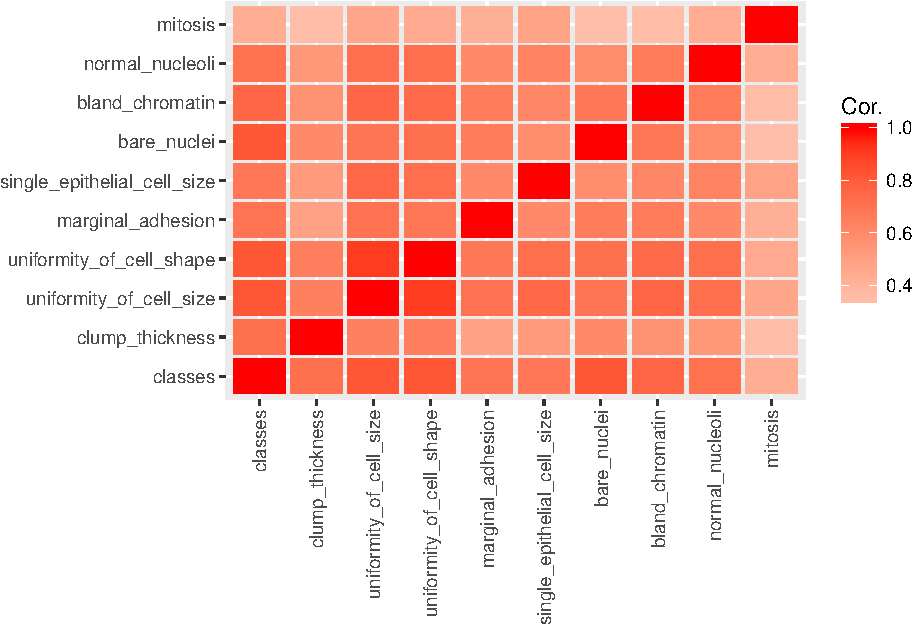
\includegraphics{webinar_code_files/figure-latex/corr_plot-1.pdf}

\paragraph{Training, validation and test
data}\label{training-validation-and-test-data-1}

Now we can use the \emph{h2o.splitFrame()} function to split the data
into training, validation and test data. Here, I am using 70\% for
training and 15\% each for validation and testing. We could also just
split the data into two sections, a training and test set but when we
have sufficient samples, it is a good idea to evaluate model performance
on an independent test set on top of training with a validation set.
Because we can easily overfit a model, we want to get an idea about how
generalizable it is - this we can only assess by looking at how well it
works on previously unknown data.

I am also defining response and feature column names now.

\begin{Shaded}
\begin{Highlighting}[]
\NormalTok{splits <-}\StringTok{ }\KeywordTok{h2o.splitFrame}\NormalTok{(bc_data_hf, }
                         \DataTypeTok{ratios =} \KeywordTok{c}\NormalTok{(}\FloatTok{0.7}\NormalTok{, }\FloatTok{0.15}\NormalTok{), }
                         \DataTypeTok{seed =} \DecValTok{1}\NormalTok{)}

\NormalTok{train <-}\StringTok{ }\NormalTok{splits[[}\DecValTok{1}\NormalTok{]]}
\NormalTok{valid <-}\StringTok{ }\NormalTok{splits[[}\DecValTok{2}\NormalTok{]]}
\NormalTok{test <-}\StringTok{ }\NormalTok{splits[[}\DecValTok{3}\NormalTok{]]}

\NormalTok{response <-}\StringTok{ "classes"}
\NormalTok{features <-}\StringTok{ }\KeywordTok{setdiff}\NormalTok{(}\KeywordTok{colnames}\NormalTok{(train), response)}
\end{Highlighting}
\end{Shaded}

\begin{Shaded}
\begin{Highlighting}[]
\KeywordTok{summary}\NormalTok{(train$classes, }\DataTypeTok{exact_quantiles =} \OtherTok{TRUE}\NormalTok{)}
\end{Highlighting}
\end{Shaded}

\begin{verbatim}
##  classes       
##  benign   :317 
##  malignant:174
\end{verbatim}

\begin{Shaded}
\begin{Highlighting}[]
\KeywordTok{summary}\NormalTok{(valid$classes, }\DataTypeTok{exact_quantiles =} \OtherTok{TRUE}\NormalTok{)}
\end{Highlighting}
\end{Shaded}

\begin{verbatim}
##  classes      
##  benign   :71 
##  malignant:35
\end{verbatim}

\begin{Shaded}
\begin{Highlighting}[]
\KeywordTok{summary}\NormalTok{(test$classes, }\DataTypeTok{exact_quantiles =} \OtherTok{TRUE}\NormalTok{)}
\end{Highlighting}
\end{Shaded}

\begin{verbatim}
##  classes      
##  benign   :70 
##  malignant:32
\end{verbatim}

We can also run a PCA on the training data, using the
\emph{h2o.prcomp()} function to calculate the singular value
decomposition of the Gram matrix with the power method.

\begin{Shaded}
\begin{Highlighting}[]
\NormalTok{pca <-}\StringTok{ }\KeywordTok{h2o.prcomp}\NormalTok{(}\DataTypeTok{training_frame =} \NormalTok{train,}
           \DataTypeTok{x =} \NormalTok{features,}
           \DataTypeTok{validation_frame =} \NormalTok{valid,}
           \DataTypeTok{transform =} \StringTok{"NORMALIZE"}\NormalTok{,}
           \DataTypeTok{impute_missing =} \OtherTok{TRUE}\NormalTok{,}
           \DataTypeTok{k =} \DecValTok{3}\NormalTok{,}
           \DataTypeTok{seed =} \DecValTok{42}\NormalTok{)}
\end{Highlighting}
\end{Shaded}

\begin{verbatim}
## 
  |                                                                       
  |                                                                 |   0%
  |                                                                       
  |=================================================================| 100%
\end{verbatim}

\begin{Shaded}
\begin{Highlighting}[]
\NormalTok{eigenvec <-}\StringTok{ }\KeywordTok{as.data.frame}\NormalTok{(pca@model$eigenvectors)}
\NormalTok{eigenvec$label <-}\StringTok{ }\NormalTok{features}

\KeywordTok{library}\NormalTok{(ggrepel)}
\KeywordTok{ggplot}\NormalTok{(eigenvec, }\KeywordTok{aes}\NormalTok{(}\DataTypeTok{x =} \NormalTok{pc1, }\DataTypeTok{y =} \NormalTok{pc2, }\DataTypeTok{label =} \NormalTok{label)) +}
\StringTok{  }\KeywordTok{geom_point}\NormalTok{(}\DataTypeTok{color =} \StringTok{"navy"}\NormalTok{, }\DataTypeTok{alpha =} \FloatTok{0.7}\NormalTok{) +}
\StringTok{  }\KeywordTok{geom_text_repel}\NormalTok{()}
\end{Highlighting}
\end{Shaded}

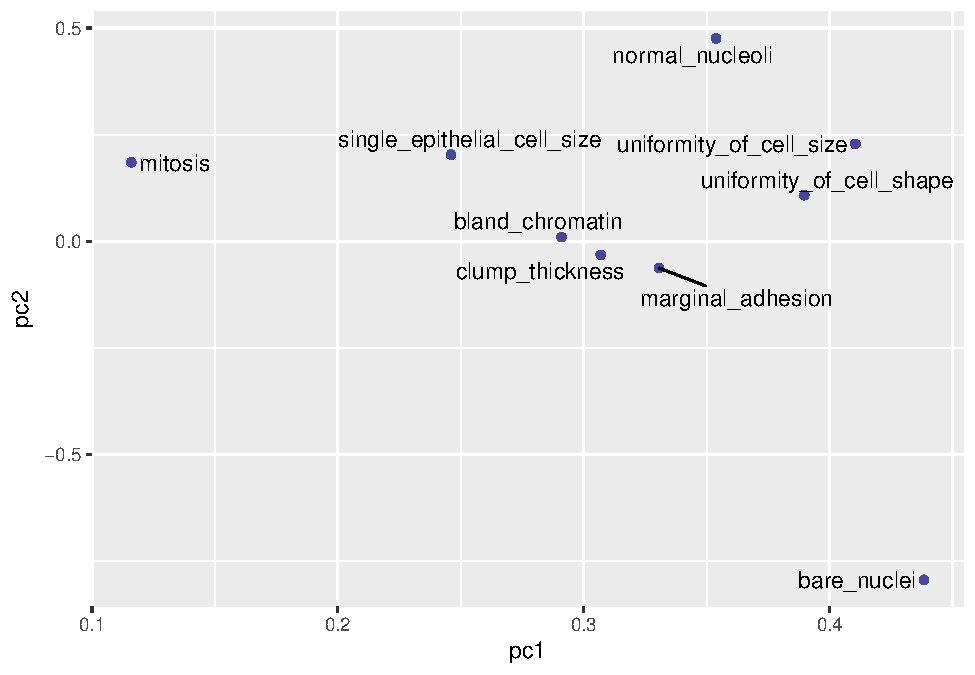
\includegraphics{webinar_code_files/figure-latex/pca_features-1.pdf}

\paragraph{Classification}\label{classification-1}

Of course, you need quite a bit of experience and intuition to hit on a
good combination of parameters. That's why it usually makes sense to do
a grid search for hyper-parameter tuning. Hyper-parameter tuning with
grid search allows us to test different combinations of hyper-parameters
and find one with improved accuracy.

Keep in mind though, that hyper-parameter tuning can only improve the
model so much without overfitting. If you can't achieve sufficient
accuracy, the input features might simply not be adequate for the
predictions you are trying to model. It might be necessary to go back to
the original features and try e.g.~feature engineering methods.

We can use the \texttt{h2o.grid()} function to perform a Random Grid
Search (RGS). We could also test all possible combinations of parameters
with Cartesian Grid or exhaustive search, but RGS is much faster when we
have a large number of possible combinations and usually finds
sufficiently accurate models.

For RGS, we first define a set of hyper-parameters and search criteria
to fine-tune our models. Because there are many hyper-parameters, each
with a range of possible values, we want to find an (ideally) optimal
combination to maximize our model's accuracy. We can also specify how
long we want to run the grid search for. Based on the results of each
model tested in the grid, we can choose the one with the highest
accuracy or best performance for the question on hand.

\subparagraph{Random Forest}\label{random-forest}

\begin{Shaded}
\begin{Highlighting}[]
\NormalTok{hyper_params <-}\StringTok{ }\KeywordTok{list}\NormalTok{(}
                     \DataTypeTok{ntrees =} \KeywordTok{c}\NormalTok{(}\DecValTok{25}\NormalTok{, }\DecValTok{50}\NormalTok{, }\DecValTok{75}\NormalTok{, }\DecValTok{100}\NormalTok{),}
                     \DataTypeTok{max_depth =} \KeywordTok{c}\NormalTok{(}\DecValTok{10}\NormalTok{, }\DecValTok{20}\NormalTok{, }\DecValTok{30}\NormalTok{),}
                     \DataTypeTok{min_rows =} \KeywordTok{c}\NormalTok{(}\DecValTok{1}\NormalTok{, }\DecValTok{3}\NormalTok{, }\DecValTok{5}\NormalTok{)}
                     \NormalTok{)}

\NormalTok{search_criteria <-}\StringTok{ }\KeywordTok{list}\NormalTok{(}
                        \DataTypeTok{strategy =} \StringTok{"RandomDiscrete"}\NormalTok{, }
                        \DataTypeTok{max_models =} \DecValTok{50}\NormalTok{,}
                        \DataTypeTok{max_runtime_secs =} \DecValTok{360}\NormalTok{,}
                        \DataTypeTok{stopping_rounds =} \DecValTok{5}\NormalTok{,          }
                        \DataTypeTok{stopping_metric =} \StringTok{"AUC"}\NormalTok{,      }
                        \DataTypeTok{stopping_tolerance =} \FloatTok{0.0005}\NormalTok{,}
                        \DataTypeTok{seed =} \DecValTok{42}
                        \NormalTok{)}
\end{Highlighting}
\end{Shaded}

\begin{Shaded}
\begin{Highlighting}[]
\NormalTok{rf_grid <-}\StringTok{ }\KeywordTok{h2o.grid}\NormalTok{(}\DataTypeTok{algorithm =} \StringTok{"randomForest"}\NormalTok{, }\CommentTok{# h2o.randomForest, }
                                                \CommentTok{# alternatively h2o.gbm for Gradient boosting trees}
                    \DataTypeTok{x =} \NormalTok{features,}
                    \DataTypeTok{y =} \NormalTok{response,}
                    \DataTypeTok{grid_id =} \StringTok{"rf_grid"}\NormalTok{,}
                    \DataTypeTok{training_frame =} \NormalTok{train,}
                    \DataTypeTok{validation_frame =} \NormalTok{valid,}
                    \DataTypeTok{nfolds =} \DecValTok{25}\NormalTok{,                           }
                    \DataTypeTok{fold_assignment =} \StringTok{"Stratified"}\NormalTok{,}
                    \DataTypeTok{hyper_params =} \NormalTok{hyper_params,}
                    \DataTypeTok{search_criteria =} \NormalTok{search_criteria,}
                    \DataTypeTok{seed =} \DecValTok{42}
                    \NormalTok{)}
\end{Highlighting}
\end{Shaded}

We now want to extract the best model from the grid model list. What
makes a model \emph{the best} depends on the question you want to
address with it: in some cases, the model with highest AUC is the most
suitable, or the one with the lowest mean squared error, etc. We first
use the \texttt{h2o.getGrid()} function to sort all models by the
quality metric we choose (depending on the metric, you want it ordered
by descending or ascending values). We can then get the model that's the
first in the list to work with further. This model's hyper-parameters
can be found with \texttt{best\_model@allparameters}. You can now work
with your best model as with any regular model in \textbf{h2o}.

\begin{Shaded}
\begin{Highlighting}[]
\CommentTok{# performance metrics where smaller is better -> order with decreasing = FALSE}
\NormalTok{sort_options_1 <-}\StringTok{ }\KeywordTok{c}\NormalTok{(}\StringTok{"mean_per_class_error"}\NormalTok{, }\StringTok{"mse"}\NormalTok{, }\StringTok{"err"}\NormalTok{, }\StringTok{"logloss"}\NormalTok{)}

\NormalTok{for (sort_by_1 in sort_options_1) \{}
  
  \NormalTok{grid <-}\StringTok{ }\KeywordTok{h2o.getGrid}\NormalTok{(}\StringTok{"rf_grid"}\NormalTok{, }\DataTypeTok{sort_by =} \NormalTok{sort_by_1, }\DataTypeTok{decreasing =} \OtherTok{FALSE}\NormalTok{)}
  
  \NormalTok{model_ids <-}\StringTok{ }\NormalTok{grid@model_ids}
  \NormalTok{best_model <-}\StringTok{ }\KeywordTok{h2o.getModel}\NormalTok{(model_ids[[}\DecValTok{1}\NormalTok{]])}
  
  \KeywordTok{h2o.saveModel}\NormalTok{(best_model, }\DataTypeTok{path=}\StringTok{"models"}\NormalTok{, }\DataTypeTok{force =} \OtherTok{TRUE}\NormalTok{)}
  
\NormalTok{\}}


\CommentTok{# performance metrics where bigger is better -> order with decreasing = TRUE}
\NormalTok{sort_options_2 <-}\StringTok{ }\KeywordTok{c}\NormalTok{(}\StringTok{"auc"}\NormalTok{, }\StringTok{"precision"}\NormalTok{, }\StringTok{"accuracy"}\NormalTok{, }\StringTok{"recall"}\NormalTok{, }\StringTok{"specificity"}\NormalTok{)}

\NormalTok{for (sort_by_2 in sort_options_2) \{}
  
  \NormalTok{grid <-}\StringTok{ }\KeywordTok{h2o.getGrid}\NormalTok{(}\StringTok{"rf_grid"}\NormalTok{, }\DataTypeTok{sort_by =} \NormalTok{sort_by_2, }\DataTypeTok{decreasing =} \OtherTok{TRUE}\NormalTok{)}
  
  \NormalTok{model_ids <-}\StringTok{ }\NormalTok{grid@model_ids}
  \NormalTok{best_model <-}\StringTok{ }\KeywordTok{h2o.getModel}\NormalTok{(model_ids[[}\DecValTok{1}\NormalTok{]])}
  
  \KeywordTok{h2o.saveModel}\NormalTok{(best_model, }\DataTypeTok{path =} \StringTok{"models"}\NormalTok{, }\DataTypeTok{force =} \OtherTok{TRUE}\NormalTok{)}
  
\NormalTok{\}}
\end{Highlighting}
\end{Shaded}

The ultimate performance test for our model will be it's prediction
accuracy on the test set it hasn't seen before. Here, I will compare the
AUC and mean squared error for each best model from before. You could of
course look at any other quality metric that is most appropriate for
your model.

\begin{Shaded}
\begin{Highlighting}[]
\NormalTok{files <-}\StringTok{ }\KeywordTok{list.files}\NormalTok{(}\DataTypeTok{path =} \StringTok{"models"}\NormalTok{)}
\NormalTok{rf_models <-}\StringTok{ }\NormalTok{files[}\KeywordTok{grep}\NormalTok{(}\StringTok{"rf_grid_model"}\NormalTok{, files)]}

\NormalTok{for (model_id in rf_models) \{}
  
  \CommentTok{#path <- paste0("U:\textbackslash{}\textbackslash{}Github_blog\textbackslash{}\textbackslash{}Webinar\textbackslash{}\textbackslash{}Webinar_ML_for_disease\textbackslash{}\textbackslash{}models\textbackslash{}\textbackslash{}", model_id)}
  \NormalTok{path <-}\StringTok{ }\KeywordTok{paste0}\NormalTok{(}\StringTok{"/Users/Shirin/Documents/Github/Webinar_ML_for_disease/models/"}\NormalTok{, model_id)}
  \NormalTok{best_model <-}\StringTok{ }\KeywordTok{h2o.loadModel}\NormalTok{(path)}
  \NormalTok{mse_auc_test <-}\StringTok{ }\KeywordTok{data.frame}\NormalTok{(}\DataTypeTok{model_id =} \NormalTok{model_id, }
                             \DataTypeTok{mse =} \KeywordTok{h2o.mse}\NormalTok{(}\KeywordTok{h2o.performance}\NormalTok{(best_model, test)),}
                             \DataTypeTok{auc =} \KeywordTok{h2o.auc}\NormalTok{(}\KeywordTok{h2o.performance}\NormalTok{(best_model, test)))}
  
  \NormalTok{if (model_id ==}\StringTok{ }\NormalTok{rf_models[[}\DecValTok{1}\NormalTok{]]) \{}
    
    \NormalTok{mse_auc_test_comb <-}\StringTok{ }\NormalTok{mse_auc_test}
    
  \NormalTok{\} else \{}
    
    \NormalTok{mse_auc_test_comb <-}\StringTok{ }\KeywordTok{rbind}\NormalTok{(mse_auc_test_comb, mse_auc_test)}
    
  \NormalTok{\}}
\NormalTok{\}}

\NormalTok{mse_auc_test_comb %>%}
\StringTok{  }\KeywordTok{gather}\NormalTok{(x, y, mse:auc) %>%}
\StringTok{  }\KeywordTok{ggplot}\NormalTok{(}\KeywordTok{aes}\NormalTok{(}\DataTypeTok{x =} \NormalTok{model_id, }\DataTypeTok{y =} \NormalTok{y, }\DataTypeTok{fill =} \NormalTok{model_id)) +}
\StringTok{    }\KeywordTok{facet_grid}\NormalTok{(x ~}\StringTok{ }\NormalTok{., }\DataTypeTok{scales =} \StringTok{"free"}\NormalTok{) +}
\StringTok{    }\KeywordTok{geom_bar}\NormalTok{(}\DataTypeTok{stat =} \StringTok{"identity"}\NormalTok{, }\DataTypeTok{alpha =} \FloatTok{0.8}\NormalTok{, }\DataTypeTok{position =} \StringTok{"dodge"}\NormalTok{) +}
\StringTok{    }\KeywordTok{scale_fill_brewer}\NormalTok{(}\DataTypeTok{palette =} \StringTok{"Set1"}\NormalTok{) +}
\StringTok{    }\KeywordTok{theme}\NormalTok{(}\DataTypeTok{axis.text.x =} \KeywordTok{element_text}\NormalTok{(}\DataTypeTok{angle =} \DecValTok{45}\NormalTok{, }\DataTypeTok{vjust =} \DecValTok{1}\NormalTok{, }\DataTypeTok{hjust =} \DecValTok{1}\NormalTok{),}
          \DataTypeTok{plot.margin =} \KeywordTok{unit}\NormalTok{(}\KeywordTok{c}\NormalTok{(}\FloatTok{0.5}\NormalTok{, }\DecValTok{0}\NormalTok{, }\DecValTok{0}\NormalTok{, }\FloatTok{1.5}\NormalTok{), }\StringTok{"cm"}\NormalTok{)) +}
\StringTok{    }\KeywordTok{labs}\NormalTok{(}\DataTypeTok{x =} \StringTok{""}\NormalTok{, }\DataTypeTok{y =} \StringTok{"value"}\NormalTok{, }\DataTypeTok{fill =} \StringTok{""}\NormalTok{)}
\end{Highlighting}
\end{Shaded}

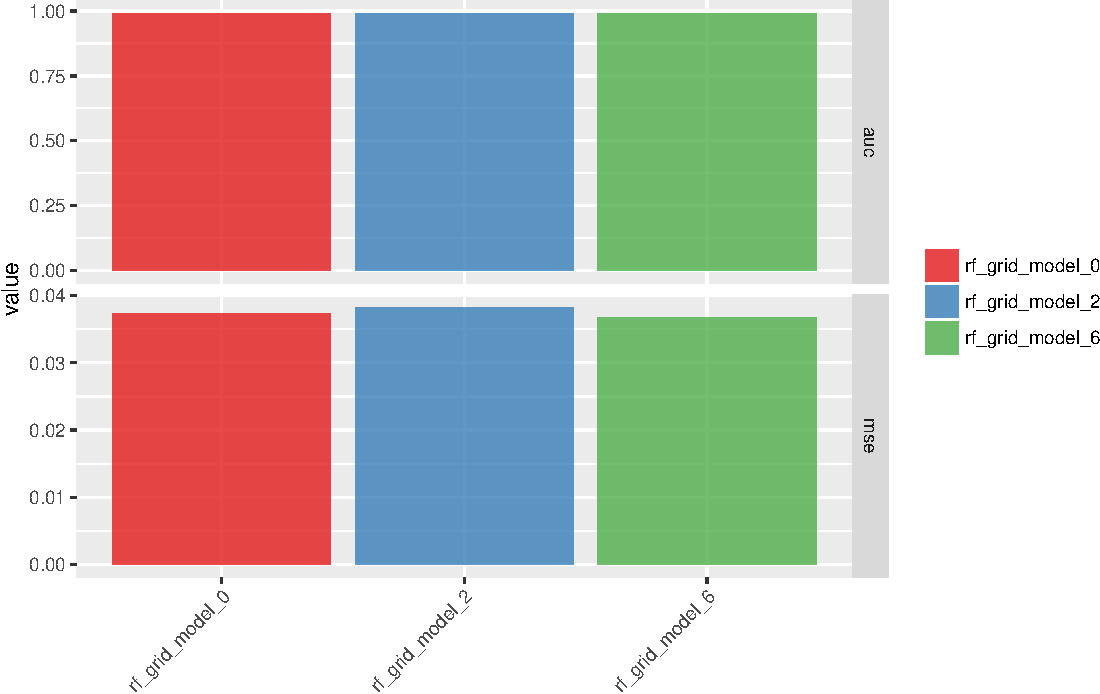
\includegraphics{webinar_code_files/figure-latex/auc_mse-1.pdf}

I will then create a dataframe with predictions for each test sample
with all best models. As in last week's post, I want to compare the
default predictions with stringent predictions.

\begin{Shaded}
\begin{Highlighting}[]
\NormalTok{for (model_id in rf_models) \{}
  
  \NormalTok{best_model <-}\StringTok{ }\KeywordTok{h2o.getModel}\NormalTok{(model_id)}
  
  \NormalTok{finalRf_predictions <-}\StringTok{ }\KeywordTok{data.frame}\NormalTok{(}\DataTypeTok{model_id =} \KeywordTok{rep}\NormalTok{(best_model@model_id, }
                                                   \KeywordTok{nrow}\NormalTok{(test)),}
                                    \DataTypeTok{actual =} \KeywordTok{as.vector}\NormalTok{(test$classes), }
                                    \KeywordTok{as.data.frame}\NormalTok{(}\KeywordTok{h2o.predict}\NormalTok{(}\DataTypeTok{object =} \NormalTok{best_model, }
                                                              \DataTypeTok{newdata =} \NormalTok{test)))}
  
  \NormalTok{finalRf_predictions$accurate <-}\StringTok{ }\KeywordTok{ifelse}\NormalTok{(finalRf_predictions$actual ==}\StringTok{ }\NormalTok{finalRf_predictions$predict, }
                                         \StringTok{"yes"}\NormalTok{, }\StringTok{"no"}\NormalTok{)}
  
  \NormalTok{finalRf_predictions$predict_stringent <-}\StringTok{ }\KeywordTok{ifelse}\NormalTok{(finalRf_predictions$benign >}\StringTok{ }\FloatTok{0.8}\NormalTok{, }
                                                  \StringTok{"benign"}\NormalTok{, }
                                                  \KeywordTok{ifelse}\NormalTok{(finalRf_predictions$malignant >}\StringTok{ }\FloatTok{0.8}\NormalTok{, }
                                                         \StringTok{"malignant"}\NormalTok{, }\StringTok{"uncertain"}\NormalTok{))}
  
  \NormalTok{finalRf_predictions$accurate_stringent <-}\StringTok{ }\KeywordTok{ifelse}\NormalTok{(finalRf_predictions$actual ==}\StringTok{ }\NormalTok{finalRf_predictions$predict_stringent, }
                                                   \StringTok{"yes"}\NormalTok{, }
                                         \KeywordTok{ifelse}\NormalTok{(finalRf_predictions$predict_stringent ==}\StringTok{ "uncertain"}\NormalTok{, }
                                                \StringTok{"na"}\NormalTok{, }\StringTok{"no"}\NormalTok{))}
  
  \NormalTok{if (model_id ==}\StringTok{ }\NormalTok{rf_models[[}\DecValTok{1}\NormalTok{]]) \{}
    
    \NormalTok{finalRf_predictions_comb <-}\StringTok{ }\NormalTok{finalRf_predictions}
    
  \NormalTok{\} else \{}
    
    \NormalTok{finalRf_predictions_comb <-}\StringTok{ }\KeywordTok{rbind}\NormalTok{(finalRf_predictions_comb, finalRf_predictions)}
    
  \NormalTok{\}}
\NormalTok{\}}
\end{Highlighting}
\end{Shaded}

\begin{verbatim}
## 
  |                                                                       
  |                                                                 |   0%
  |                                                                       
  |=================================================================| 100%
## 
  |                                                                       
  |                                                                 |   0%
  |                                                                       
  |=================================================================| 100%
## 
  |                                                                       
  |                                                                 |   0%
  |                                                                       
  |=================================================================| 100%
\end{verbatim}

\begin{Shaded}
\begin{Highlighting}[]
\NormalTok{finalRf_predictions_comb %>%}
\StringTok{  }\KeywordTok{ggplot}\NormalTok{(}\KeywordTok{aes}\NormalTok{(}\DataTypeTok{x =} \NormalTok{actual, }\DataTypeTok{fill =} \NormalTok{accurate)) +}
\StringTok{    }\KeywordTok{geom_bar}\NormalTok{(}\DataTypeTok{position =} \StringTok{"dodge"}\NormalTok{) +}
\StringTok{    }\KeywordTok{scale_fill_brewer}\NormalTok{(}\DataTypeTok{palette =} \StringTok{"Set1"}\NormalTok{) +}
\StringTok{    }\KeywordTok{facet_wrap}\NormalTok{(~}\StringTok{ }\NormalTok{model_id, }\DataTypeTok{ncol =} \DecValTok{3}\NormalTok{) +}
\StringTok{    }\KeywordTok{labs}\NormalTok{(}\DataTypeTok{fill =} \StringTok{"Were}\CharTok{\textbackslash{}n}\StringTok{predictions}\CharTok{\textbackslash{}n}\StringTok{accurate?"}\NormalTok{,}
         \DataTypeTok{title =} \StringTok{"Default predictions"}\NormalTok{)}
\end{Highlighting}
\end{Shaded}

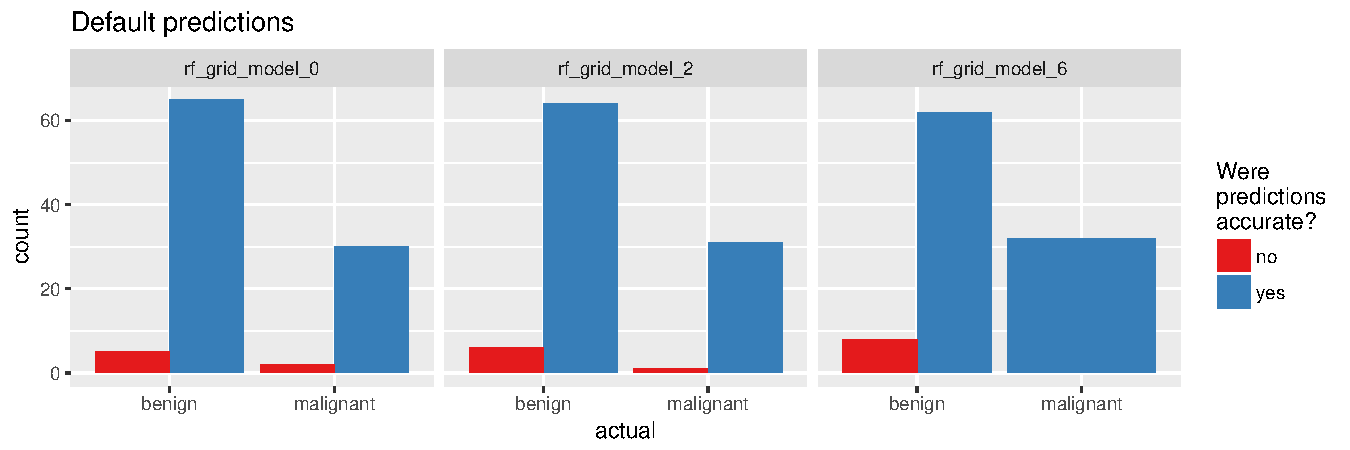
\includegraphics{webinar_code_files/figure-latex/final_predictions_rf-1.pdf}

\begin{Shaded}
\begin{Highlighting}[]
\NormalTok{finalRf_predictions_comb %>%}
\StringTok{  }\KeywordTok{subset}\NormalTok{(accurate_stringent !=}\StringTok{ "na"}\NormalTok{) %>%}
\StringTok{  }\KeywordTok{ggplot}\NormalTok{(}\KeywordTok{aes}\NormalTok{(}\DataTypeTok{x =} \NormalTok{actual, }\DataTypeTok{fill =} \NormalTok{accurate_stringent)) +}
\StringTok{    }\KeywordTok{geom_bar}\NormalTok{(}\DataTypeTok{position =} \StringTok{"dodge"}\NormalTok{) +}
\StringTok{    }\KeywordTok{scale_fill_brewer}\NormalTok{(}\DataTypeTok{palette =} \StringTok{"Set1"}\NormalTok{) +}
\StringTok{    }\KeywordTok{facet_wrap}\NormalTok{(~}\StringTok{ }\NormalTok{model_id, }\DataTypeTok{ncol =} \DecValTok{3}\NormalTok{) +}
\StringTok{    }\KeywordTok{labs}\NormalTok{(}\DataTypeTok{fill =} \StringTok{"Were}\CharTok{\textbackslash{}n}\StringTok{predictions}\CharTok{\textbackslash{}n}\StringTok{accurate?"}\NormalTok{,}
         \DataTypeTok{title =} \StringTok{"Stringent predictions"}\NormalTok{)}
\end{Highlighting}
\end{Shaded}

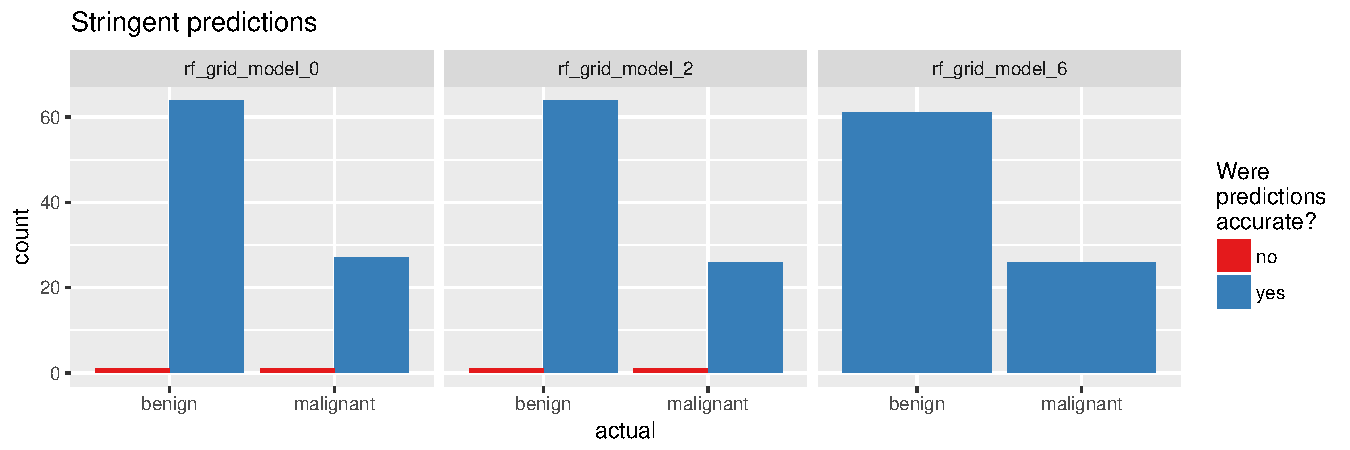
\includegraphics{webinar_code_files/figure-latex/final_predictions_rf-2.pdf}

With predictions made by different models, we can see where each model
performs best. This obviously corresponds with the quality metric we
chose to define the best model. Stringent prediction thresholds reduced
the number of false predictions but of course also the number of
predictions made at all.

\begin{Shaded}
\begin{Highlighting}[]
\CommentTok{#rf_model <- h2o.loadModel("U:\textbackslash{}\textbackslash{}Github_blog\textbackslash{}\textbackslash{}Webinar\textbackslash{}\textbackslash{}Webinar_ML_for_disease\textbackslash{}\textbackslash{}models\textbackslash{}\textbackslash{}rf_grid_model_6")}
\NormalTok{rf_model <-}\StringTok{ }\KeywordTok{h2o.loadModel}\NormalTok{(}\StringTok{"models/rf_grid_model_6"}\NormalTok{)}
\CommentTok{#summary(rf_model)}
\end{Highlighting}
\end{Shaded}

\begin{Shaded}
\begin{Highlighting}[]
\KeywordTok{h2o.varimp_plot}\NormalTok{(rf_model)}
\end{Highlighting}
\end{Shaded}

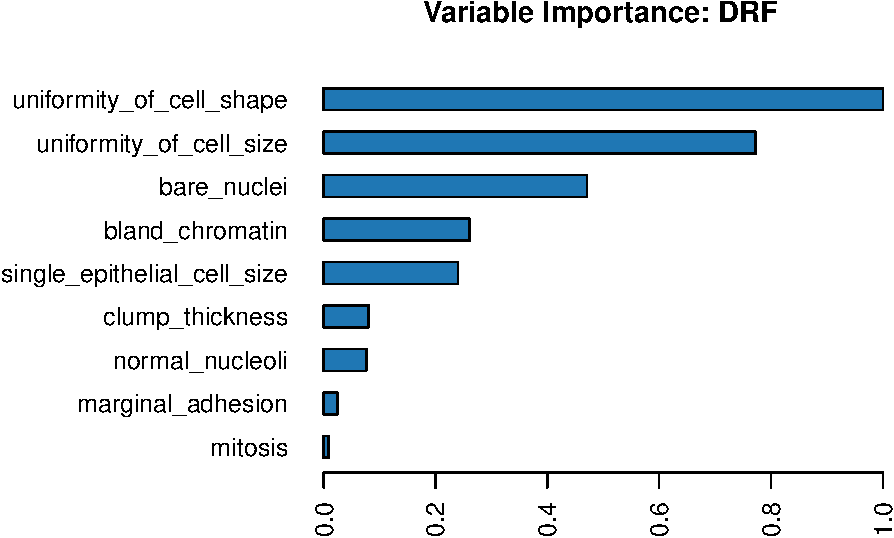
\includegraphics{webinar_code_files/figure-latex/unnamed-chunk-41-1.pdf}

\begin{Shaded}
\begin{Highlighting}[]
\CommentTok{#h2o.varimp(rf_model)}
\end{Highlighting}
\end{Shaded}

One performance metric we are interested in is the mean per class error
for training and validation data.

\begin{Shaded}
\begin{Highlighting}[]
\KeywordTok{h2o.mean_per_class_error}\NormalTok{(rf_model, }\DataTypeTok{train =} \OtherTok{TRUE}\NormalTok{, }\DataTypeTok{valid =} \OtherTok{TRUE}\NormalTok{, }\DataTypeTok{xval =} \OtherTok{TRUE}\NormalTok{)}
\end{Highlighting}
\end{Shaded}

\begin{verbatim}
##       train       valid        xval 
## 0.024674571 0.007042254 0.023097284
\end{verbatim}

The confusion matrix tells us, how many classes have been predicted
correctly and how many predictions were accurate. Here, we see the
errors in predictions on validation data

\begin{Shaded}
\begin{Highlighting}[]
\KeywordTok{h2o.confusionMatrix}\NormalTok{(rf_model, }\DataTypeTok{valid =} \OtherTok{TRUE}\NormalTok{)}
\end{Highlighting}
\end{Shaded}

\begin{verbatim}
## Confusion Matrix (vertical: actual; across: predicted)  for max f1 @ threshold = 0.293125896751881:
##           benign malignant    Error    Rate
## benign        70         1 0.014085   =1/71
## malignant      0        35 0.000000   =0/35
## Totals        70        36 0.009434  =1/106
\end{verbatim}

We can also plot the classification error.

\begin{Shaded}
\begin{Highlighting}[]
\KeywordTok{plot}\NormalTok{(rf_model,}
     \DataTypeTok{timestep =} \StringTok{"number_of_trees"}\NormalTok{,}
     \DataTypeTok{metric =} \StringTok{"classification_error"}\NormalTok{)}
\end{Highlighting}
\end{Shaded}

\begin{center}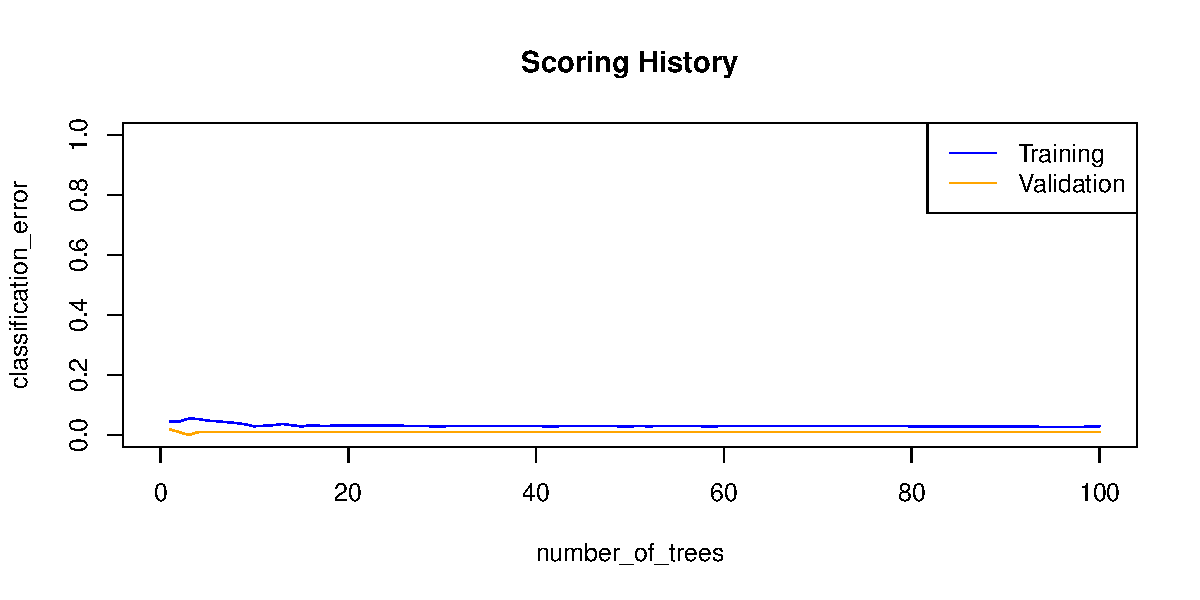
\includegraphics{webinar_code_files/figure-latex/unnamed-chunk-44-1} \end{center}

Next to the classification error, we are usually interested in the
logistic loss (negative log-likelihood or log loss). It describes the
sum of errors for each sample in the training or validation data or the
negative logarithm of the likelihood of error for a given prediction/
classification. Simply put, the lower the loss, the better the model (if
we ignore potential overfitting).

\begin{Shaded}
\begin{Highlighting}[]
\KeywordTok{plot}\NormalTok{(rf_model,}
     \DataTypeTok{timestep =} \StringTok{"number_of_trees"}\NormalTok{,}
     \DataTypeTok{metric =} \StringTok{"logloss"}\NormalTok{)}
\end{Highlighting}
\end{Shaded}

\begin{center}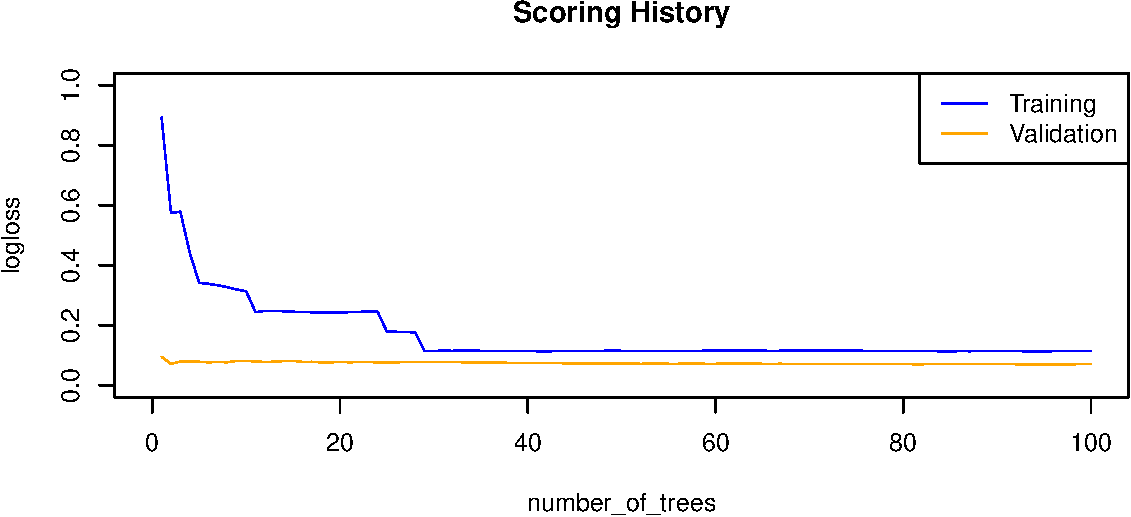
\includegraphics{webinar_code_files/figure-latex/unnamed-chunk-45-1} \end{center}

\begin{Shaded}
\begin{Highlighting}[]
\KeywordTok{plot}\NormalTok{(rf_model,}
     \DataTypeTok{timestep =} \StringTok{"number_of_trees"}\NormalTok{,}
     \DataTypeTok{metric =} \StringTok{"AUC"}\NormalTok{)}
\end{Highlighting}
\end{Shaded}

\begin{center}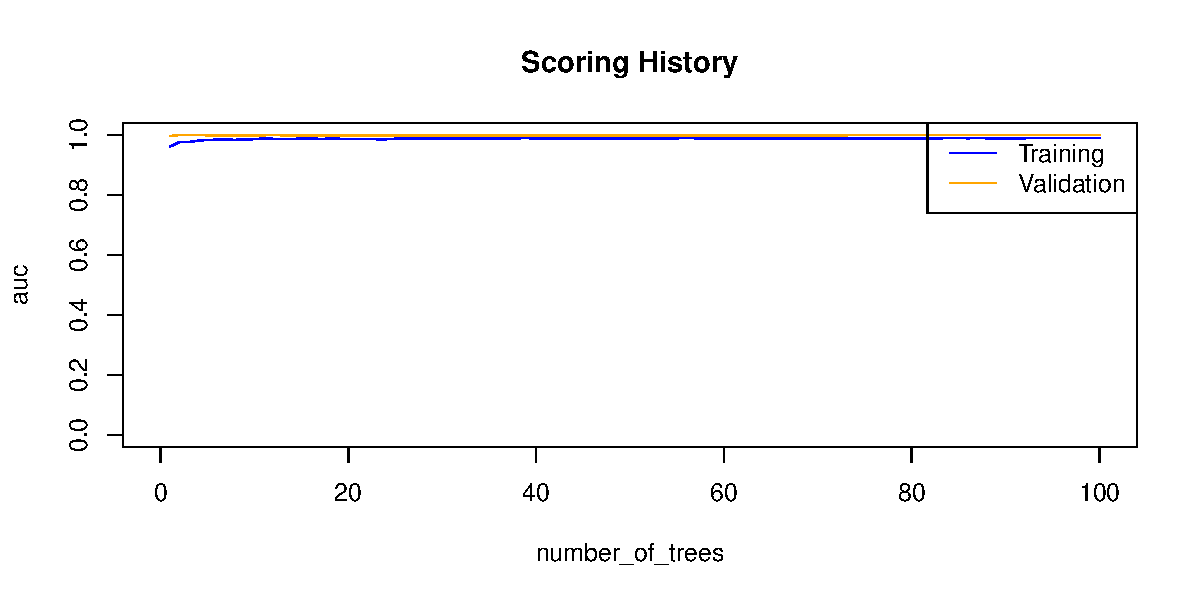
\includegraphics{webinar_code_files/figure-latex/unnamed-chunk-46-1} \end{center}

We can also plot the mean squared error (MSE). The MSE tells us the
average of the prediction errors squared, i.e.~the estimator's variance
and bias. The closer to zero, the better a model.

\begin{Shaded}
\begin{Highlighting}[]
\KeywordTok{plot}\NormalTok{(rf_model,}
     \DataTypeTok{timestep =} \StringTok{"number_of_trees"}\NormalTok{,}
     \DataTypeTok{metric =} \StringTok{"rmse"}\NormalTok{)}
\end{Highlighting}
\end{Shaded}

\begin{center}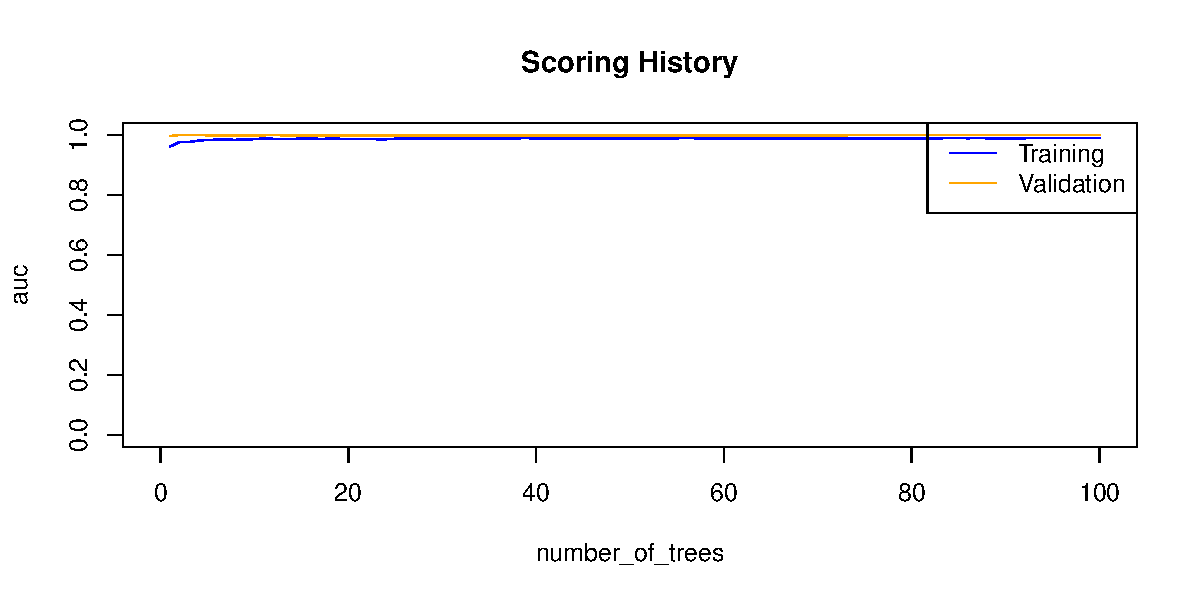
\includegraphics{webinar_code_files/figure-latex/unnamed-chunk-47-1} \end{center}

Next, we want to know the area under the curve (AUC). AUC is an
important metric for measuring binary classification model performances.
It gives the area under the curve, i.e.~the integral, of true positive
vs false positive rates. The closer to 1, the better a model. AUC is
especially useful, when we have unbalanced datasets (meaning datasets
where one class is much more common than the other), because it is
independent of class labels.

\begin{Shaded}
\begin{Highlighting}[]
\KeywordTok{h2o.auc}\NormalTok{(rf_model, }\DataTypeTok{train =} \OtherTok{TRUE}\NormalTok{)}
\end{Highlighting}
\end{Shaded}

\begin{verbatim}
## [1] 0.989521
\end{verbatim}

\begin{Shaded}
\begin{Highlighting}[]
\KeywordTok{h2o.auc}\NormalTok{(rf_model, }\DataTypeTok{valid =} \OtherTok{TRUE}\NormalTok{)}
\end{Highlighting}
\end{Shaded}

\begin{verbatim}
## [1] 0.9995976
\end{verbatim}

\begin{Shaded}
\begin{Highlighting}[]
\KeywordTok{h2o.auc}\NormalTok{(rf_model, }\DataTypeTok{xval =} \OtherTok{TRUE}\NormalTok{)}
\end{Highlighting}
\end{Shaded}

\begin{verbatim}
## [1] 0.9890496
\end{verbatim}

Now that we have a good idea about model performance on validation data,
we want to know how it performed on unseen test data. A good model
should find an optimal balance between accuracy on training and test
data. A model that has 0\% error on the training data but 40\% error on
the test data is in effect useless. It overfit on the training data and
is thus not able to generalize to unknown data.

\begin{Shaded}
\begin{Highlighting}[]
\NormalTok{perf <-}\StringTok{ }\KeywordTok{h2o.performance}\NormalTok{(rf_model, test)}
\NormalTok{perf}
\end{Highlighting}
\end{Shaded}

\begin{verbatim}
## H2OBinomialMetrics: drf
## 
## MSE:  0.03673598
## RMSE:  0.1916663
## LogLoss:  0.1158835
## Mean Per-Class Error:  0.0625
## AUC:  0.990625
## Gini:  0.98125
## 
## Confusion Matrix (vertical: actual; across: predicted) for F1-optimal threshold:
##           benign malignant    Error    Rate
## benign        70         0 0.000000   =0/70
## malignant      4        28 0.125000   =4/32
## Totals        74        28 0.039216  =4/102
## 
## Maximum Metrics: Maximum metrics at their respective thresholds
##                         metric threshold    value idx
## 1                       max f1  0.735027 0.933333  25
## 2                       max f2  0.294222 0.952381  37
## 3                 max f0point5  0.735027 0.972222  25
## 4                 max accuracy  0.735027 0.960784  25
## 5                max precision  1.000000 1.000000   0
## 6                   max recall  0.294222 1.000000  37
## 7              max specificity  1.000000 1.000000   0
## 8             max absolute_mcc  0.735027 0.909782  25
## 9   max min_per_class_accuracy  0.424524 0.937500  31
## 10 max mean_per_class_accuracy  0.294222 0.942857  37
## 
## Gains/Lift Table: Extract with `h2o.gainsLift(<model>, <data>)` or `h2o.gainsLift(<model>, valid=<T/F>, xval=<T/F>)`
\end{verbatim}

Plotting the test performance's AUC plot shows us approximately how good
the predictions are.

\begin{Shaded}
\begin{Highlighting}[]
\KeywordTok{plot}\NormalTok{(perf)}
\end{Highlighting}
\end{Shaded}

\begin{center}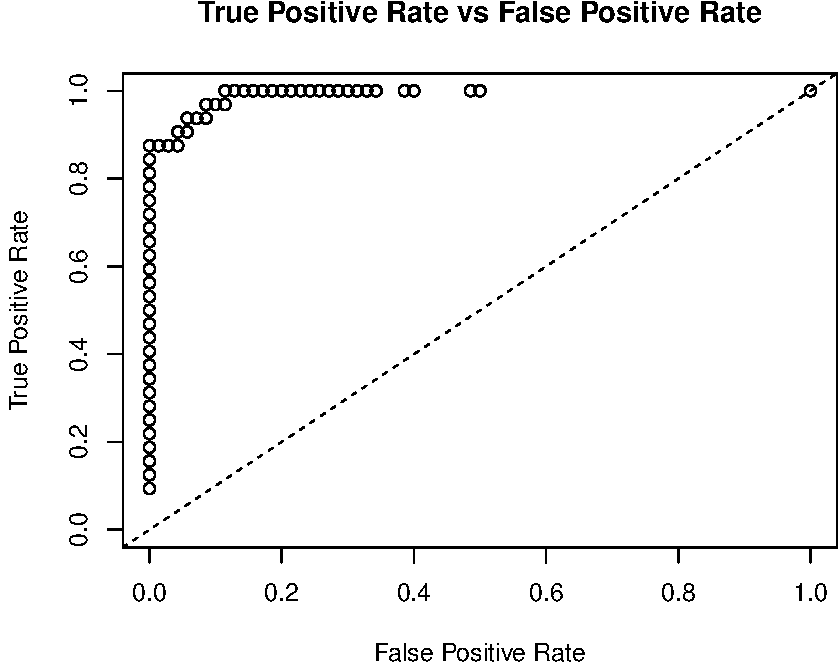
\includegraphics{webinar_code_files/figure-latex/auc_curve-1} \end{center}

We also want to know the log loss, MSE and AUC values, as well as other
model metrics for the test data:

\begin{Shaded}
\begin{Highlighting}[]
\KeywordTok{h2o.logloss}\NormalTok{(perf)}
\end{Highlighting}
\end{Shaded}

\begin{verbatim}
## [1] 0.1158835
\end{verbatim}

\begin{Shaded}
\begin{Highlighting}[]
\KeywordTok{h2o.mse}\NormalTok{(perf)}
\end{Highlighting}
\end{Shaded}

\begin{verbatim}
## [1] 0.03673598
\end{verbatim}

\begin{Shaded}
\begin{Highlighting}[]
\KeywordTok{h2o.auc}\NormalTok{(perf)}
\end{Highlighting}
\end{Shaded}

\begin{verbatim}
## [1] 0.990625
\end{verbatim}

\begin{Shaded}
\begin{Highlighting}[]
\KeywordTok{head}\NormalTok{(}\KeywordTok{h2o.metric}\NormalTok{(perf))}
\end{Highlighting}
\end{Shaded}

\begin{verbatim}
## Metrics for Thresholds: Binomial metrics as a function of classification thresholds
##   threshold       f1       f2 f0point5 accuracy precision   recall
## 1  1.000000 0.171429 0.114504 0.340909 0.715686  1.000000 0.093750
## 2  0.998333 0.222222 0.151515 0.416667 0.725490  1.000000 0.125000
## 3  0.998000 0.270270 0.187970 0.480769 0.735294  1.000000 0.156250
## 4  0.997222 0.315789 0.223881 0.535714 0.745098  1.000000 0.187500
## 5  0.996210 0.358974 0.259259 0.583333 0.754902  1.000000 0.218750
## 6  0.994048 0.400000 0.294118 0.625000 0.764706  1.000000 0.250000
##   specificity absolute_mcc min_per_class_accuracy mean_per_class_accuracy
## 1    1.000000     0.257464               0.093750                0.546875
## 2    1.000000     0.298807               0.125000                0.562500
## 3    1.000000     0.335794               0.156250                0.578125
## 4    1.000000     0.369755               0.187500                0.593750
## 5    1.000000     0.401478               0.218750                0.609375
## 6    1.000000     0.431474               0.250000                0.625000
##   tns fns fps tps      tnr      fnr      fpr      tpr idx
## 1  70  29   0   3 1.000000 0.906250 0.000000 0.093750   0
## 2  70  28   0   4 1.000000 0.875000 0.000000 0.125000   1
## 3  70  27   0   5 1.000000 0.843750 0.000000 0.156250   2
## 4  70  26   0   6 1.000000 0.812500 0.000000 0.187500   3
## 5  70  25   0   7 1.000000 0.781250 0.000000 0.218750   4
## 6  70  24   0   8 1.000000 0.750000 0.000000 0.250000   5
\end{verbatim}

The final predictions with probabilities can be extracted with the
\emph{h2o.predict()} function. Beware though, that the number of correct
and wrong classifications can be slightly different from the confusion
matrix above. Here, I combine the predictions with the actual test
diagnoses and classes into a data frame. For plotting I also want to
have a column, that tells me whether the predictions were correct. By
default, a prediction probability above 0.5 will get scored as a
prediction for the respective category. I find it often makes sense to
be more stringent with this, though and set a higher threshold.
Therefore, I am creating another column with stringent predictions,
where I only count predictions that were made with more than 80\%
probability. Everything that does not fall within this range gets scored
as ``uncertain''. For these stringent predictions, I am also creating a
column that tells me whether they were accurate.

\begin{Shaded}
\begin{Highlighting}[]
\NormalTok{finalRf_predictions <-}\StringTok{ }\KeywordTok{data.frame}\NormalTok{(}\DataTypeTok{actual =} \KeywordTok{as.vector}\NormalTok{(test$classes), }
                                  \KeywordTok{as.data.frame}\NormalTok{(}\KeywordTok{h2o.predict}\NormalTok{(}\DataTypeTok{object =} \NormalTok{rf_model, }\DataTypeTok{newdata =} \NormalTok{test)))}
\end{Highlighting}
\end{Shaded}

\begin{verbatim}
## 
  |                                                                       
  |                                                                 |   0%
  |                                                                       
  |=================================================================| 100%
\end{verbatim}

\begin{Shaded}
\begin{Highlighting}[]
\NormalTok{finalRf_predictions$accurate <-}\StringTok{ }\KeywordTok{ifelse}\NormalTok{(finalRf_predictions$actual ==}\StringTok{ }\NormalTok{finalRf_predictions$predict, }\StringTok{"yes"}\NormalTok{, }\StringTok{"no"}\NormalTok{)}

\NormalTok{finalRf_predictions$predict_stringent <-}\StringTok{ }\KeywordTok{ifelse}\NormalTok{(finalRf_predictions$benign >}\StringTok{ }\FloatTok{0.8}\NormalTok{, }\StringTok{"benign"}\NormalTok{, }
                                                \KeywordTok{ifelse}\NormalTok{(finalRf_predictions$malignant >}\StringTok{ }\FloatTok{0.8}\NormalTok{, }\StringTok{"malignant"}\NormalTok{, }\StringTok{"uncertain"}\NormalTok{))}
\NormalTok{finalRf_predictions$accurate_stringent <-}\StringTok{ }\KeywordTok{ifelse}\NormalTok{(finalRf_predictions$actual ==}\StringTok{ }\NormalTok{finalRf_predictions$predict_stringent, }\StringTok{"yes"}\NormalTok{, }
                                       \KeywordTok{ifelse}\NormalTok{(finalRf_predictions$predict_stringent ==}\StringTok{ "uncertain"}\NormalTok{, }\StringTok{"na"}\NormalTok{, }\StringTok{"no"}\NormalTok{))}

\NormalTok{finalRf_predictions %>%}
\StringTok{  }\KeywordTok{group_by}\NormalTok{(actual, predict) %>%}
\StringTok{  }\NormalTok{dplyr::}\KeywordTok{summarise}\NormalTok{(}\DataTypeTok{n =} \KeywordTok{n}\NormalTok{())}
\end{Highlighting}
\end{Shaded}

\begin{verbatim}
## Source: local data frame [3 x 3]
## Groups: actual [?]
## 
##      actual   predict     n
##      <fctr>    <fctr> <int>
## 1    benign    benign    62
## 2    benign malignant     8
## 3 malignant malignant    32
\end{verbatim}

\begin{Shaded}
\begin{Highlighting}[]
\NormalTok{finalRf_predictions %>%}
\StringTok{  }\KeywordTok{group_by}\NormalTok{(actual, predict_stringent) %>%}
\StringTok{  }\NormalTok{dplyr::}\KeywordTok{summarise}\NormalTok{(}\DataTypeTok{n =} \KeywordTok{n}\NormalTok{())}
\end{Highlighting}
\end{Shaded}

\begin{verbatim}
## Source: local data frame [4 x 3]
## Groups: actual [?]
## 
##      actual predict_stringent     n
##      <fctr>             <chr> <int>
## 1    benign            benign    61
## 2    benign         uncertain     9
## 3 malignant         malignant    26
## 4 malignant         uncertain     6
\end{verbatim}

\begin{Shaded}
\begin{Highlighting}[]
\NormalTok{finalRf_predictions %>%}
\StringTok{  }\KeywordTok{ggplot}\NormalTok{(}\KeywordTok{aes}\NormalTok{(}\DataTypeTok{x =} \NormalTok{actual, }\DataTypeTok{fill =} \NormalTok{accurate)) +}
\StringTok{    }\KeywordTok{geom_bar}\NormalTok{(}\DataTypeTok{position =} \StringTok{"dodge"}\NormalTok{) +}
\StringTok{    }\KeywordTok{scale_fill_brewer}\NormalTok{(}\DataTypeTok{palette =} \StringTok{"Set1"}\NormalTok{) +}
\StringTok{    }\KeywordTok{labs}\NormalTok{(}\DataTypeTok{fill =} \StringTok{"Were}\CharTok{\textbackslash{}n}\StringTok{predictions}\CharTok{\textbackslash{}n}\StringTok{accurate?"}\NormalTok{,}
         \DataTypeTok{title =} \StringTok{"Default predictions"}\NormalTok{)}
\end{Highlighting}
\end{Shaded}

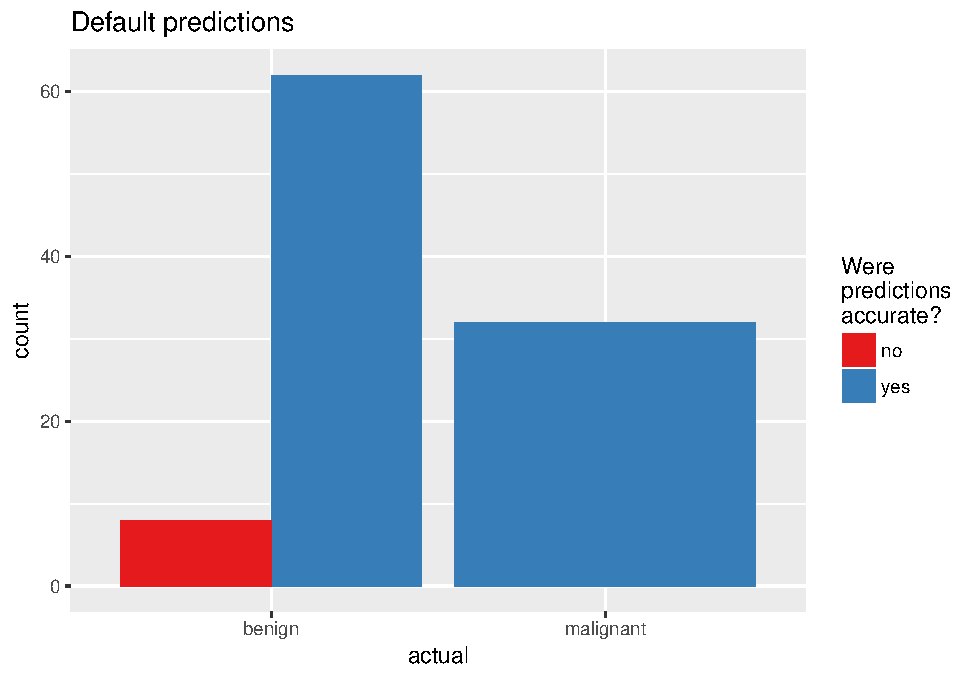
\includegraphics{webinar_code_files/figure-latex/unnamed-chunk-52-1.pdf}

\begin{Shaded}
\begin{Highlighting}[]
\NormalTok{finalRf_predictions %>%}
\StringTok{  }\KeywordTok{subset}\NormalTok{(accurate_stringent !=}\StringTok{ "na"}\NormalTok{) %>%}
\StringTok{  }\KeywordTok{ggplot}\NormalTok{(}\KeywordTok{aes}\NormalTok{(}\DataTypeTok{x =} \NormalTok{actual, }\DataTypeTok{fill =} \NormalTok{accurate_stringent)) +}
\StringTok{    }\KeywordTok{geom_bar}\NormalTok{(}\DataTypeTok{position =} \StringTok{"dodge"}\NormalTok{) +}
\StringTok{    }\KeywordTok{scale_fill_brewer}\NormalTok{(}\DataTypeTok{palette =} \StringTok{"Set1"}\NormalTok{) +}
\StringTok{    }\KeywordTok{labs}\NormalTok{(}\DataTypeTok{fill =} \StringTok{"Were}\CharTok{\textbackslash{}n}\StringTok{predictions}\CharTok{\textbackslash{}n}\StringTok{accurate?"}\NormalTok{,}
         \DataTypeTok{title =} \StringTok{"Stringent predictions"}\NormalTok{)}
\end{Highlighting}
\end{Shaded}

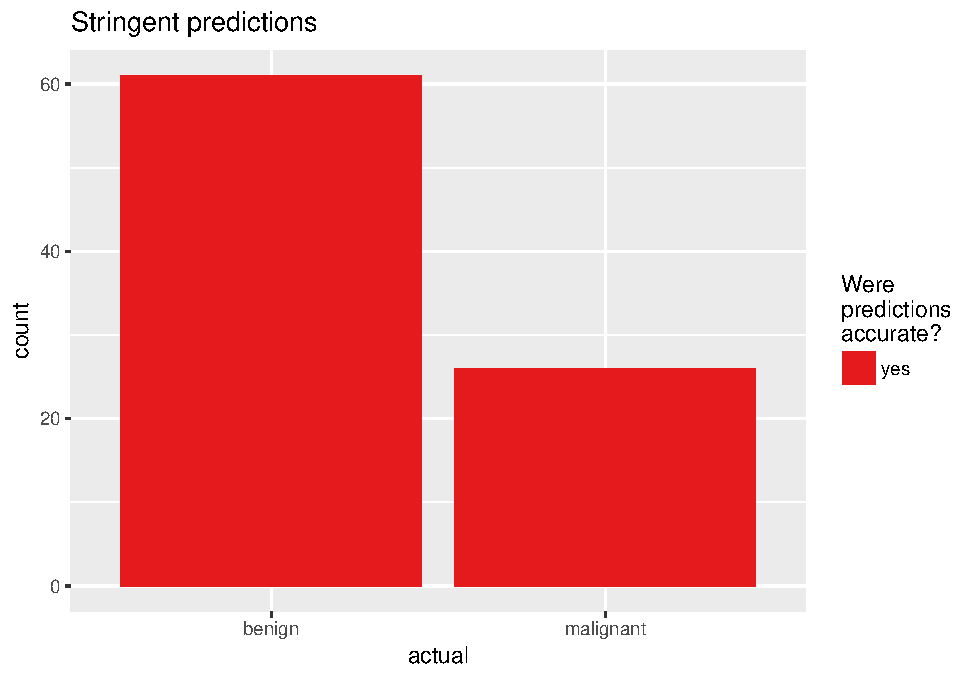
\includegraphics{webinar_code_files/figure-latex/unnamed-chunk-52-2.pdf}

\subparagraph{Deep learning with neural
networks}\label{deep-learning-with-neural-networks}

Deep learning with neural networks is arguably one of the most rapidly
growing applications of machine learning and AI today. They allow
building complex models that consist of multiple hidden layers within
artifiical networks and are able to find non-linear patterns in
unstructured data. Deep neural networks are usually feed-forward, which
means that each layer feeds its output to subsequent layers, but
recurrent or feed-back neural networks can also be built. Feed-forward
neural networks are also called multilayer perceptrons (MLPs).

We can specify quite a few parameters, like

\begin{itemize}
\item
  \textbf{Cross-validation}: Cross validation can tell us the training
  and validation errors for each model. The final model will be
  overwritten with the best model, if we don't specify otherwise.
\item
  \textbf{Adaptive learning rate}: For deep learning with h2o, we by
  default use stochastic gradient descent optimization with an an
  adaptive learning rate. The two corresponding parameters \emph{rho}
  and \emph{epsilon} help us find global (or near enough) optima.
\item
  \textbf{Epochs}: Increasing the number of epochs (one full training
  cycle on all training samples) can increase model performance, but we
  also run the risk of overfitting. To determine the optimal number of
  epochs, we need to use early stopping.
\item
  \textbf{Early stopping}: By default, early stopping is enabled. This
  means that training will be stopped when we reach a certain validation
  error to prevent overfitting. \texttt{stopping\_metric}: metric that
  we want to use as stopping criterion. \texttt{stopping\_tolerance} and
  \texttt{stopping\_rounds}: training stops when the the stopping metric
  does not improve by the stopping tolerance proportion any more
  (e.g.~by 0.05 or 5\%) for the number of consecutive rounds defined by
  stopping rounds.
\item
  \textbf{Activation Functions}: The activation function defines the
  node output relative to a given set of inputs. We want our activation
  function to be non-linear and continuously differentiable.
\end{itemize}

\texttt{Rectifier}: is the default activation function. It is the
fastest and most versatile option. It can lead to instability though and
tends to be lower in accuracy. \texttt{Tanh}: The hyperbolic tangent is
a scaled and shifted variant of the sigmoid activation function. It can
take on values from -1 to 1 and centers around 0. Tanh needs more
computational power than e.g.~the Rectifier function. \texttt{Maxout}:
is an activation function that is the max of the inputs. It is
computationally quite demanding but can produce high accuracy models.

\texttt{...WithDropout}: When we specify \texttt{with\ dropout}, a
random subset of the network is trained and the weights of all
sub-networks are averaged. It works together with the parameter
\texttt{hidden\_dropout\_ratios}, which controls the amount of layer
neurons that are randomly dropped for each hidden layer. Hidden dropout
ratios are useful for preventing overfitting on learned features.

\begin{itemize}
\item
  \textbf{Hidden layers}: Defines the number of hidden layers and the
  number of nodes per layer and are the most important hyper-parameter
  to set for deep neural networks, as they specify how many hidden
  layers and how many nodes per hidden layer the model should learn
\item
  \textbf{L1 and L2 penalties}: \texttt{L1}: lets only strong weights
  survive. \texttt{L2}: prevents any single weight from getting too big.
\item
  \textbf{Rho and Epsilon}: \texttt{rho}: similar to prior weight
  updates. \texttt{epsilon}: prevents getting stuck in local optima
\end{itemize}

\begin{Shaded}
\begin{Highlighting}[]
\NormalTok{hyper_params <-}\StringTok{ }\KeywordTok{list}\NormalTok{(}
                     \DataTypeTok{activation =} \KeywordTok{c}\NormalTok{(}\StringTok{"Rectifier"}\NormalTok{, }\StringTok{"Maxout"}\NormalTok{, }\StringTok{"Tanh"}\NormalTok{, }\StringTok{"RectifierWithDropout"}\NormalTok{, }
                                    \StringTok{"MaxoutWithDropout"}\NormalTok{, }\StringTok{"TanhWithDropout"}\NormalTok{), }
                     \DataTypeTok{hidden =} \KeywordTok{list}\NormalTok{(}\KeywordTok{c}\NormalTok{(}\DecValTok{5}\NormalTok{, }\DecValTok{5}\NormalTok{, }\DecValTok{5}\NormalTok{, }\DecValTok{5}\NormalTok{, }\DecValTok{5}\NormalTok{), }\KeywordTok{c}\NormalTok{(}\DecValTok{10}\NormalTok{, }\DecValTok{10}\NormalTok{, }\DecValTok{10}\NormalTok{, }\DecValTok{10}\NormalTok{), }\KeywordTok{c}\NormalTok{(}\DecValTok{50}\NormalTok{, }\DecValTok{50}\NormalTok{, }\DecValTok{50}\NormalTok{)),}
                     \DataTypeTok{epochs =} \KeywordTok{c}\NormalTok{(}\DecValTok{50}\NormalTok{, }\DecValTok{100}\NormalTok{, }\DecValTok{200}\NormalTok{),}
                     \DataTypeTok{l1 =} \KeywordTok{c}\NormalTok{(}\DecValTok{0}\NormalTok{, }\FloatTok{0.00001}\NormalTok{, }\FloatTok{0.0001}\NormalTok{), }
                     \DataTypeTok{l2 =} \KeywordTok{c}\NormalTok{(}\DecValTok{0}\NormalTok{, }\FloatTok{0.00001}\NormalTok{, }\FloatTok{0.0001}\NormalTok{),}
                     \DataTypeTok{rate =} \KeywordTok{c}\NormalTok{(}\DecValTok{0}\NormalTok{, }\DecValTok{01}\NormalTok{, }\FloatTok{0.005}\NormalTok{, }\FloatTok{0.001}\NormalTok{),}
                     \DataTypeTok{rate_annealing =} \KeywordTok{c}\NormalTok{(}\FloatTok{1e-8}\NormalTok{, }\FloatTok{1e-7}\NormalTok{, }\FloatTok{1e-6}\NormalTok{),}
                     \DataTypeTok{rho =} \KeywordTok{c}\NormalTok{(}\FloatTok{0.9}\NormalTok{,}\FloatTok{0.95}\NormalTok{,}\FloatTok{0.99}\NormalTok{,}\FloatTok{0.999}\NormalTok{),}
                     \DataTypeTok{epsilon =} \KeywordTok{c}\NormalTok{(}\FloatTok{1e-10}\NormalTok{,}\FloatTok{1e-8}\NormalTok{,}\FloatTok{1e-6}\NormalTok{,}\FloatTok{1e-4}\NormalTok{),}
                     \DataTypeTok{input_dropout_ratio =} \KeywordTok{c}\NormalTok{(}\DecValTok{0}\NormalTok{, }\FloatTok{0.1}\NormalTok{, }\FloatTok{0.2}\NormalTok{),}
                     \DataTypeTok{max_w2 =} \KeywordTok{c}\NormalTok{(}\DecValTok{10}\NormalTok{, }\DecValTok{100}\NormalTok{, }\DecValTok{1000}\NormalTok{, }\FloatTok{3.4028235e+38}\NormalTok{)}
                     \NormalTok{)}
\end{Highlighting}
\end{Shaded}

Now, we can train the model with combinations of hyper-parameters from
our specified stopping criteria and hyper-parameter grid.

\begin{Shaded}
\begin{Highlighting}[]
\NormalTok{dl_grid <-}\StringTok{ }\KeywordTok{h2o.grid}\NormalTok{(}\DataTypeTok{algorithm =} \StringTok{"deeplearning"}\NormalTok{, }
                    \DataTypeTok{x =} \NormalTok{features,}
                    \DataTypeTok{y =} \NormalTok{response,}
                    \DataTypeTok{grid_id =} \StringTok{"dl_grid"}\NormalTok{,}
                    \DataTypeTok{training_frame =} \NormalTok{train,}
                    \DataTypeTok{validation_frame =} \NormalTok{valid,}
                    \DataTypeTok{nfolds =} \DecValTok{25}\NormalTok{,                           }
                    \DataTypeTok{fold_assignment =} \StringTok{"Stratified"}\NormalTok{,}
                    \DataTypeTok{hyper_params =} \NormalTok{hyper_params,}
                    \DataTypeTok{search_criteria =} \NormalTok{search_criteria,}
                    \DataTypeTok{seed =} \DecValTok{42}
                    \NormalTok{)}
\end{Highlighting}
\end{Shaded}

\begin{Shaded}
\begin{Highlighting}[]
\NormalTok{grid <-}\StringTok{ }\KeywordTok{h2o.getGrid}\NormalTok{(}\StringTok{"dl_grid"}\NormalTok{, }\DataTypeTok{sort_by =} \StringTok{"auc"}\NormalTok{, }\DataTypeTok{decreasing =} \OtherTok{TRUE}\NormalTok{)}
  
\NormalTok{model_ids <-}\StringTok{ }\NormalTok{grid@model_ids}
\NormalTok{best_model <-}\StringTok{ }\KeywordTok{h2o.getModel}\NormalTok{(model_ids[[}\DecValTok{1}\NormalTok{]])}
\end{Highlighting}
\end{Shaded}

Because training can take a while, depending on how many samples,
features, nodes and hidden layers you are training on, it is a good idea
to save your model.

\begin{Shaded}
\begin{Highlighting}[]
\KeywordTok{h2o.saveModel}\NormalTok{(best_model, }\DataTypeTok{path=}\StringTok{"models"}\NormalTok{, }\DataTypeTok{force =} \OtherTok{TRUE}\NormalTok{)}
\end{Highlighting}
\end{Shaded}

We can then re-load the model again any time to check the model quality
and make predictions on new data.

\begin{Shaded}
\begin{Highlighting}[]
\NormalTok{dl_model <-}\StringTok{ }\KeywordTok{h2o.loadModel}\NormalTok{(}\StringTok{"models/dl_grid_model_8"}\NormalTok{)}
\end{Highlighting}
\end{Shaded}

We now want to know how our model performed on the validation data. The
\emph{summary()} function will give us a detailed overview of our model.
I am not showing the output here, because it is quite extensive.

\begin{Shaded}
\begin{Highlighting}[]
\NormalTok{perf <-}\StringTok{ }\KeywordTok{h2o.performance}\NormalTok{(best_model, test)}
\KeywordTok{plot}\NormalTok{(perf)}
\end{Highlighting}
\end{Shaded}

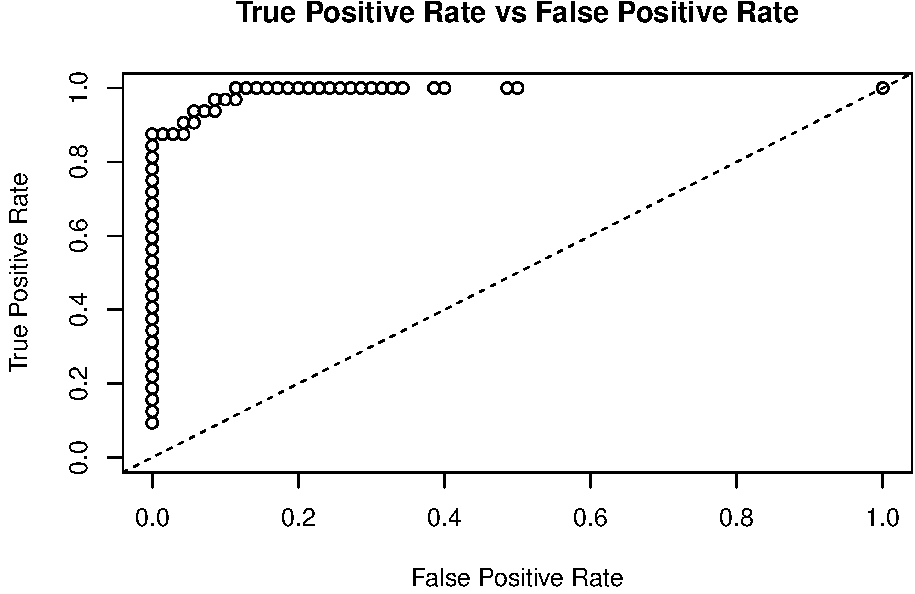
\includegraphics{webinar_code_files/figure-latex/unnamed-chunk-58-1.pdf}

\begin{Shaded}
\begin{Highlighting}[]
\KeywordTok{h2o.confusionMatrix}\NormalTok{(best_model, test)}
\end{Highlighting}
\end{Shaded}

\begin{verbatim}
## Confusion Matrix (vertical: actual; across: predicted)  for max f1 @ threshold = 0.735026690140367:
##           benign malignant    Error    Rate
## benign        70         0 0.000000   =0/70
## malignant      4        28 0.125000   =4/32
## Totals        74        28 0.039216  =4/102
\end{verbatim}

\begin{Shaded}
\begin{Highlighting}[]
\KeywordTok{h2o.shutdown}\NormalTok{()}
\end{Highlighting}
\end{Shaded}

\begin{verbatim}
## Are you sure you want to shutdown the H2O instance running at http://localhost:54321/ (Y/N)?
\end{verbatim}

\begin{center}\rule{0.5\linewidth}{\linethickness}\end{center}

If you are interested in more machine learning posts, check out
\href{https://shiring.github.io/categories.html\#machine_learning-ref}{the
category listing for \textbf{machine\_learning}}.

\begin{center}\rule{0.5\linewidth}{\linethickness}\end{center}

\begin{Shaded}
\begin{Highlighting}[]
\KeywordTok{sessionInfo}\NormalTok{()}
\end{Highlighting}
\end{Shaded}

\begin{verbatim}
## R version 3.3.2 (2016-10-31)
## Platform: x86_64-apple-darwin13.4.0 (64-bit)
## Running under: macOS Sierra 10.12.3
## 
## locale:
## [1] en_US.UTF-8/en_US.UTF-8/en_US.UTF-8/C/en_US.UTF-8/en_US.UTF-8
## 
## attached base packages:
## [1] stats4    parallel  stats     graphics  grDevices utils     datasets 
## [8] methods   base     
## 
## other attached packages:
##  [1] ggrepel_0.6.5        reshape2_1.4.2       h2o_3.10.3.6        
##  [4] corrplot_0.77        plyr_1.8.4           xgboost_0.6-4       
##  [7] randomForest_4.6-12  dplyr_0.5.0          caret_6.0-73        
## [10] lattice_0.20-34      tidyr_0.6.1          pcaGoPromoter_1.18.0
## [13] Biostrings_2.42.1    XVector_0.14.0       IRanges_2.8.1       
## [16] S4Vectors_0.12.1     BiocGenerics_0.20.0  ellipse_0.3-8       
## [19] ggplot2_2.2.1       
## 
## loaded via a namespace (and not attached):
##  [1] Rcpp_0.12.9          class_7.3-14         assertthat_0.1      
##  [4] rprojroot_1.2        digest_0.6.12        foreach_1.4.3       
##  [7] R6_2.2.0             backports_1.0.5      MatrixModels_0.4-1  
## [10] RSQLite_1.1-2        evaluate_0.10        e1071_1.6-8         
## [13] zlibbioc_1.20.0      lazyeval_0.2.0       minqa_1.2.4         
## [16] data.table_1.10.4    SparseM_1.74         car_2.1-4           
## [19] nloptr_1.0.4         Matrix_1.2-8         rmarkdown_1.3       
## [22] labeling_0.3         splines_3.3.2        lme4_1.1-12         
## [25] stringr_1.2.0        RCurl_1.95-4.8       munsell_0.4.3       
## [28] mgcv_1.8-17          htmltools_0.3.5      nnet_7.3-12         
## [31] tibble_1.2           codetools_0.2-15     MASS_7.3-45         
## [34] bitops_1.0-6         ModelMetrics_1.1.0   grid_3.3.2          
## [37] nlme_3.1-131         jsonlite_1.2         gtable_0.2.0        
## [40] DBI_0.5-1            magrittr_1.5         scales_0.4.1        
## [43] stringi_1.1.2        RColorBrewer_1.1-2   iterators_1.0.8     
## [46] tools_3.3.2          Biobase_2.34.0       pbkrtest_0.4-6      
## [49] yaml_2.1.14          AnnotationDbi_1.36.0 colorspace_1.3-2    
## [52] memoise_1.0.0        knitr_1.15.1         quantreg_5.29
\end{verbatim}


\end{document}
